\PassOptionsToPackage{unicode=true}{hyperref} % options for packages loaded elsewhere
\PassOptionsToPackage{hyphens}{url}
%
\documentclass[]{article}
\usepackage{lmodern}
\usepackage{amssymb,amsmath}
\usepackage{ifxetex,ifluatex}
\usepackage{fixltx2e} % provides \textsubscript
\ifnum 0\ifxetex 1\fi\ifluatex 1\fi=0 % if pdftex
  \usepackage[T1]{fontenc}
  \usepackage[utf8]{inputenc}
  \usepackage{textcomp} % provides euro and other symbols
\else % if luatex or xelatex
  \usepackage{unicode-math}
  \defaultfontfeatures{Ligatures=TeX,Scale=MatchLowercase}
\fi
% use upquote if available, for straight quotes in verbatim environments
\IfFileExists{upquote.sty}{\usepackage{upquote}}{}
% use microtype if available
\IfFileExists{microtype.sty}{%
\usepackage[]{microtype}
\UseMicrotypeSet[protrusion]{basicmath} % disable protrusion for tt fonts
}{}
\IfFileExists{parskip.sty}{%
\usepackage{parskip}
}{% else
\setlength{\parindent}{0pt}
\setlength{\parskip}{6pt plus 2pt minus 1pt}
}
\usepackage{hyperref}
\hypersetup{
            pdftitle={Metagenomics Occurrences on GBIF},
            pdfauthor={John Waller},
            pdfborder={0 0 0},
            breaklinks=true}
\urlstyle{same}  % don't use monospace font for urls
\usepackage[margin=1in]{geometry}
\usepackage{graphicx,grffile}
\makeatletter
\def\maxwidth{\ifdim\Gin@nat@width>\linewidth\linewidth\else\Gin@nat@width\fi}
\def\maxheight{\ifdim\Gin@nat@height>\textheight\textheight\else\Gin@nat@height\fi}
\makeatother
% Scale images if necessary, so that they will not overflow the page
% margins by default, and it is still possible to overwrite the defaults
% using explicit options in \includegraphics[width, height, ...]{}
\setkeys{Gin}{width=\maxwidth,height=\maxheight,keepaspectratio}
\setlength{\emergencystretch}{3em}  % prevent overfull lines
\providecommand{\tightlist}{%
  \setlength{\itemsep}{0pt}\setlength{\parskip}{0pt}}
\setcounter{secnumdepth}{0}
% Redefines (sub)paragraphs to behave more like sections
\ifx\paragraph\undefined\else
\let\oldparagraph\paragraph
\renewcommand{\paragraph}[1]{\oldparagraph{#1}\mbox{}}
\fi
\ifx\subparagraph\undefined\else
\let\oldsubparagraph\subparagraph
\renewcommand{\subparagraph}[1]{\oldsubparagraph{#1}\mbox{}}
\fi

% set default figure placement to htbp
\makeatletter
\def\fps@figure{htbp}
\makeatother


\title{Metagenomics Occurrences on GBIF}
\author{John Waller}
\date{2020-01-08}

\begin{document}
\maketitle

\hypertarget{most-mgnify-occurrences-are-bacteria-at-the-genus-level}{%
\section{Most mgnify occurrences are bacteria at the genus
level}\label{most-mgnify-occurrences-are-bacteria-at-the-genus-level}}

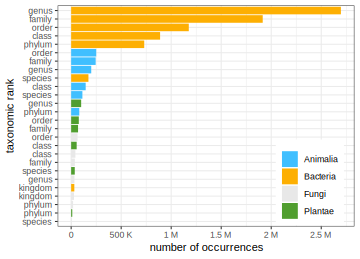
\includegraphics{/post/2020-01-08-metagenomics-occurrences-on-gbif_files/metagenomics_top_kingdoms.svg}

But there are other occurrunces of plants and animals matched to the
\textbf{species rank}.

There has been some dicussion that these type of matches might be
un-reliable.

Since it is hard to tell if something simply labeled ``Reptile'',
``Mammal'', or ``Vascular Plant'', but not resolved to a lower level is
a legitimate occurrence, I will be focusing mostly on occurrences
resovled to the \textbf{species level}.

\hypertarget{non-bacteria-in-metagenomics-datasets-have-a-high-fraction-of-geographic-outliers}{%
\section{Non-bacteria in metagenomics datasets have a high fraction of
geographic
outliers}\label{non-bacteria-in-metagenomics-datasets-have-a-high-fraction-of-geographic-outliers}}

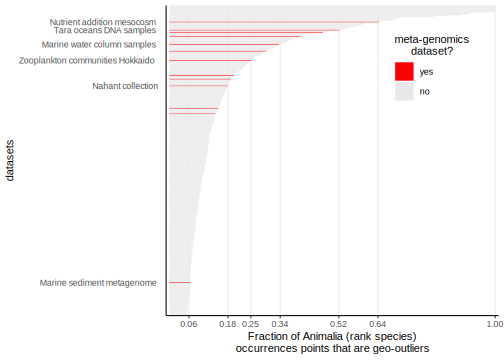
\includegraphics{/post/2020-01-08-metagenomics-occurrences-on-gbif_files/datasets_by_kingdom_percent_outliers.svg}

Occurrences from kingdom Animalia (rank species) within metagenomics
datasets, have a high fraction of geo-graphics outliers. Based on
distance outlier detection method and inter-quartile range.

While distance based outlier detection methods can be give many false
positives, it is still concerning that so many metagenomics datasets
appear close to the top!!

The datasets with a 100\% of there points as outliers are usually some
dataset occurring on an island or someplace away from the main
concetration of points.

\begin{verbatim}
mgnify

+--------------+------------+-------------+-------------------+
|       kingdom|count_mgnify|outlier_count|    percent_outlier|
+--------------+------------+-------------+-------------------+
|      Animalia|      112422|        36492|0.32459838821582965|
|      Bacteria|      172732|        36661| 0.2122420860060672|
|incertae sedis|       57370|        17042|0.29705420951716927|
|      Protozoa|       24262|        10801| 0.4451817657241777|
|     Chromista|      204177|        96280|0.47155164391679766|
|       Archaea|        2565|          162|0.06315789473684211|
|         Fungi|        7933|         1032|  0.130089499558805|
|       Plantae|       36059|        14420|0.39990016362073266|
+--------------+------------+-------------+-------------------+

inaturalist

+---------+------------+-------------+--------------------+                     
|  kingdom|count_mgnify|outlier_count|     percent_outlier|
+---------+------------+-------------+--------------------+
| Animalia|     4932243|       157663|0.031965781085806194|
| Bacteria|         670|            2|0.002985074626865...|
| Protozoa|        5078|          211| 0.04155179204411186|
|Chromista|       11039|         2283| 0.20681221125101912|
|    Fungi|      208763|        19756|  0.0946336276064245|
|  Plantae|     2818573|       202580| 0.07187324933574543|
+---------+------------+-------------+--------------------+
\end{verbatim}

\hypertarget{kingdom-animalia-outlier-examples}{%
\section{Kingdom Animalia Outlier
Examples:}\label{kingdom-animalia-outlier-examples}}

Here I go through many examples of species found within MGnify that have
likely geographic outliers. First I cover \textbf{Animals} and then move
onto \textbf{plants}.

Other {GBIF datasets} in green and {Metagenomics datasets} plotted in
red.

\hypertarget{kiwi-bird}{%
\subsubsection{Kiwi bird}\label{kiwi-bird}}

\begin{itemize}
\tightlist
\item
  link to
  \href{https://www.gbif.org/occurrence/map?taxon_key=2495145}{gbif
  map}.
\item
  The
  \href{https://www.gbif.org/occurrence/search?has_coordinate=true\&taxon_key=2495145\&advanced=1\&geometry=POLYGON((-120.67383\%2020.03906,-75.49805\%2020.03906,-75.49805\%2037.61719,-120.67383\%2037.61719,-120.67383\%2020.03906))}{two
  points} in the USA are eggs from collections.
\item
  The point off the coast of africa is a zero-zero coordinate record.
\end{itemize}

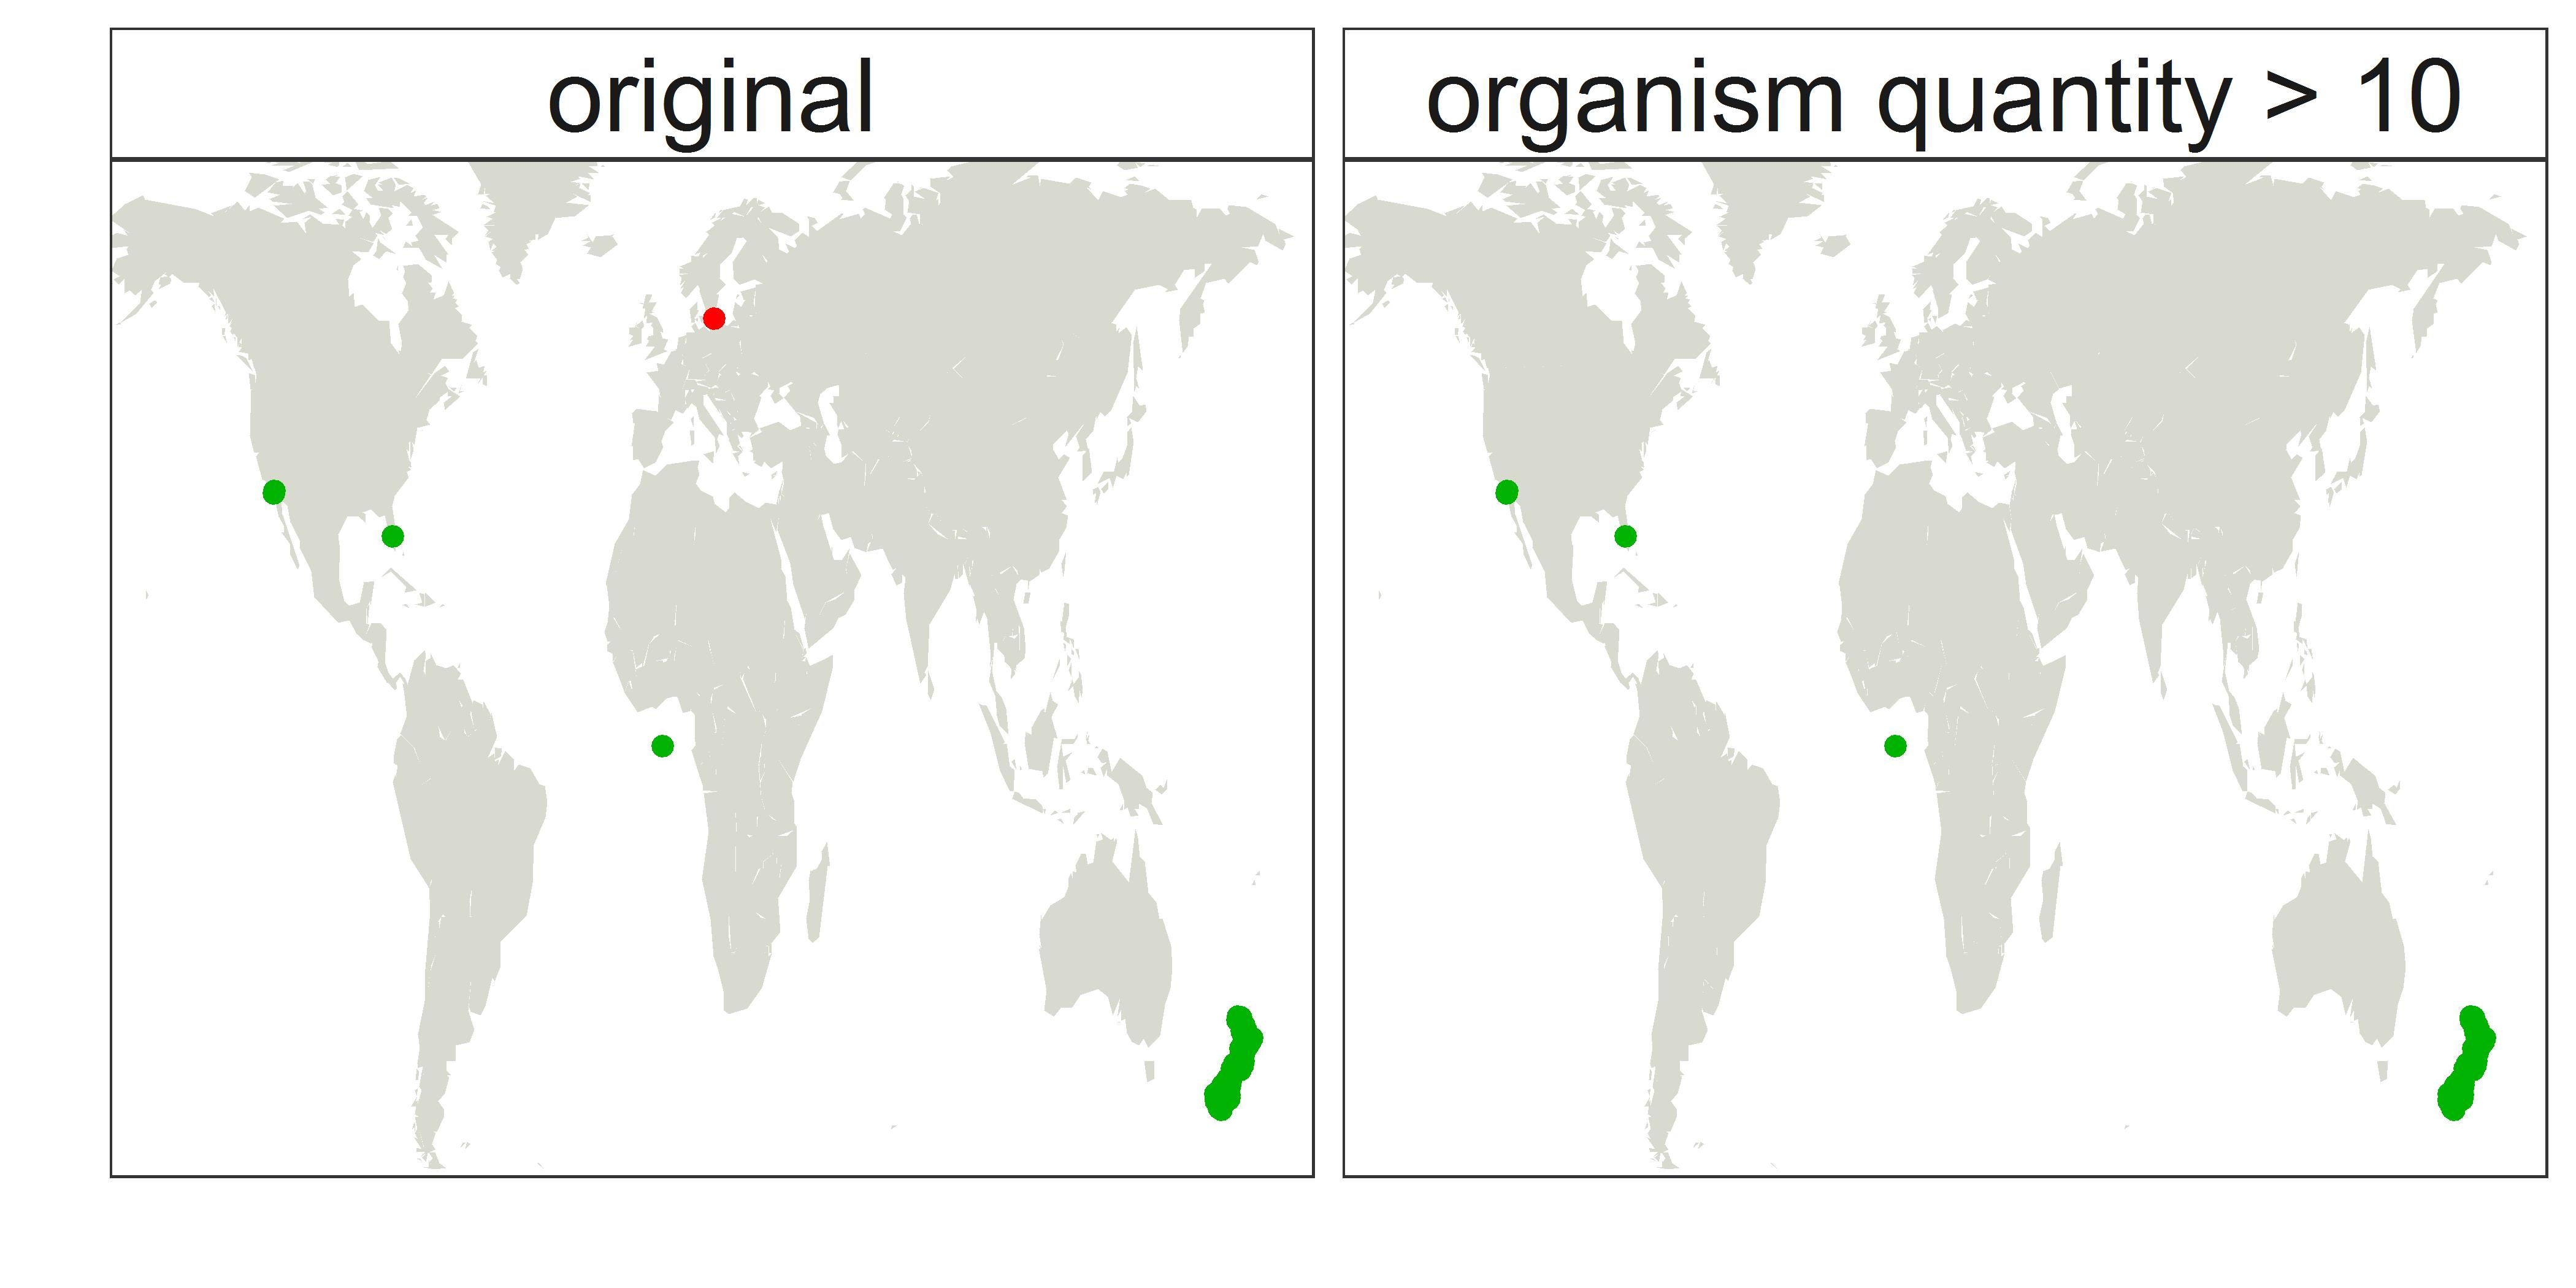
\includegraphics{/post/2020-01-08-metagenomics-occurrences-on-gbif_files/comparison_plot_2495145.jpg}

\hypertarget{lizard}{%
\subsubsection{Lizard}\label{lizard}}

\begin{itemize}
\tightlist
\item
  link to
  \href{https://www.gbif.org/occurrence/map?taxon_key=7357804}{gbif map}
\item
  The two {metagenomics points} are very suspect here.
\end{itemize}

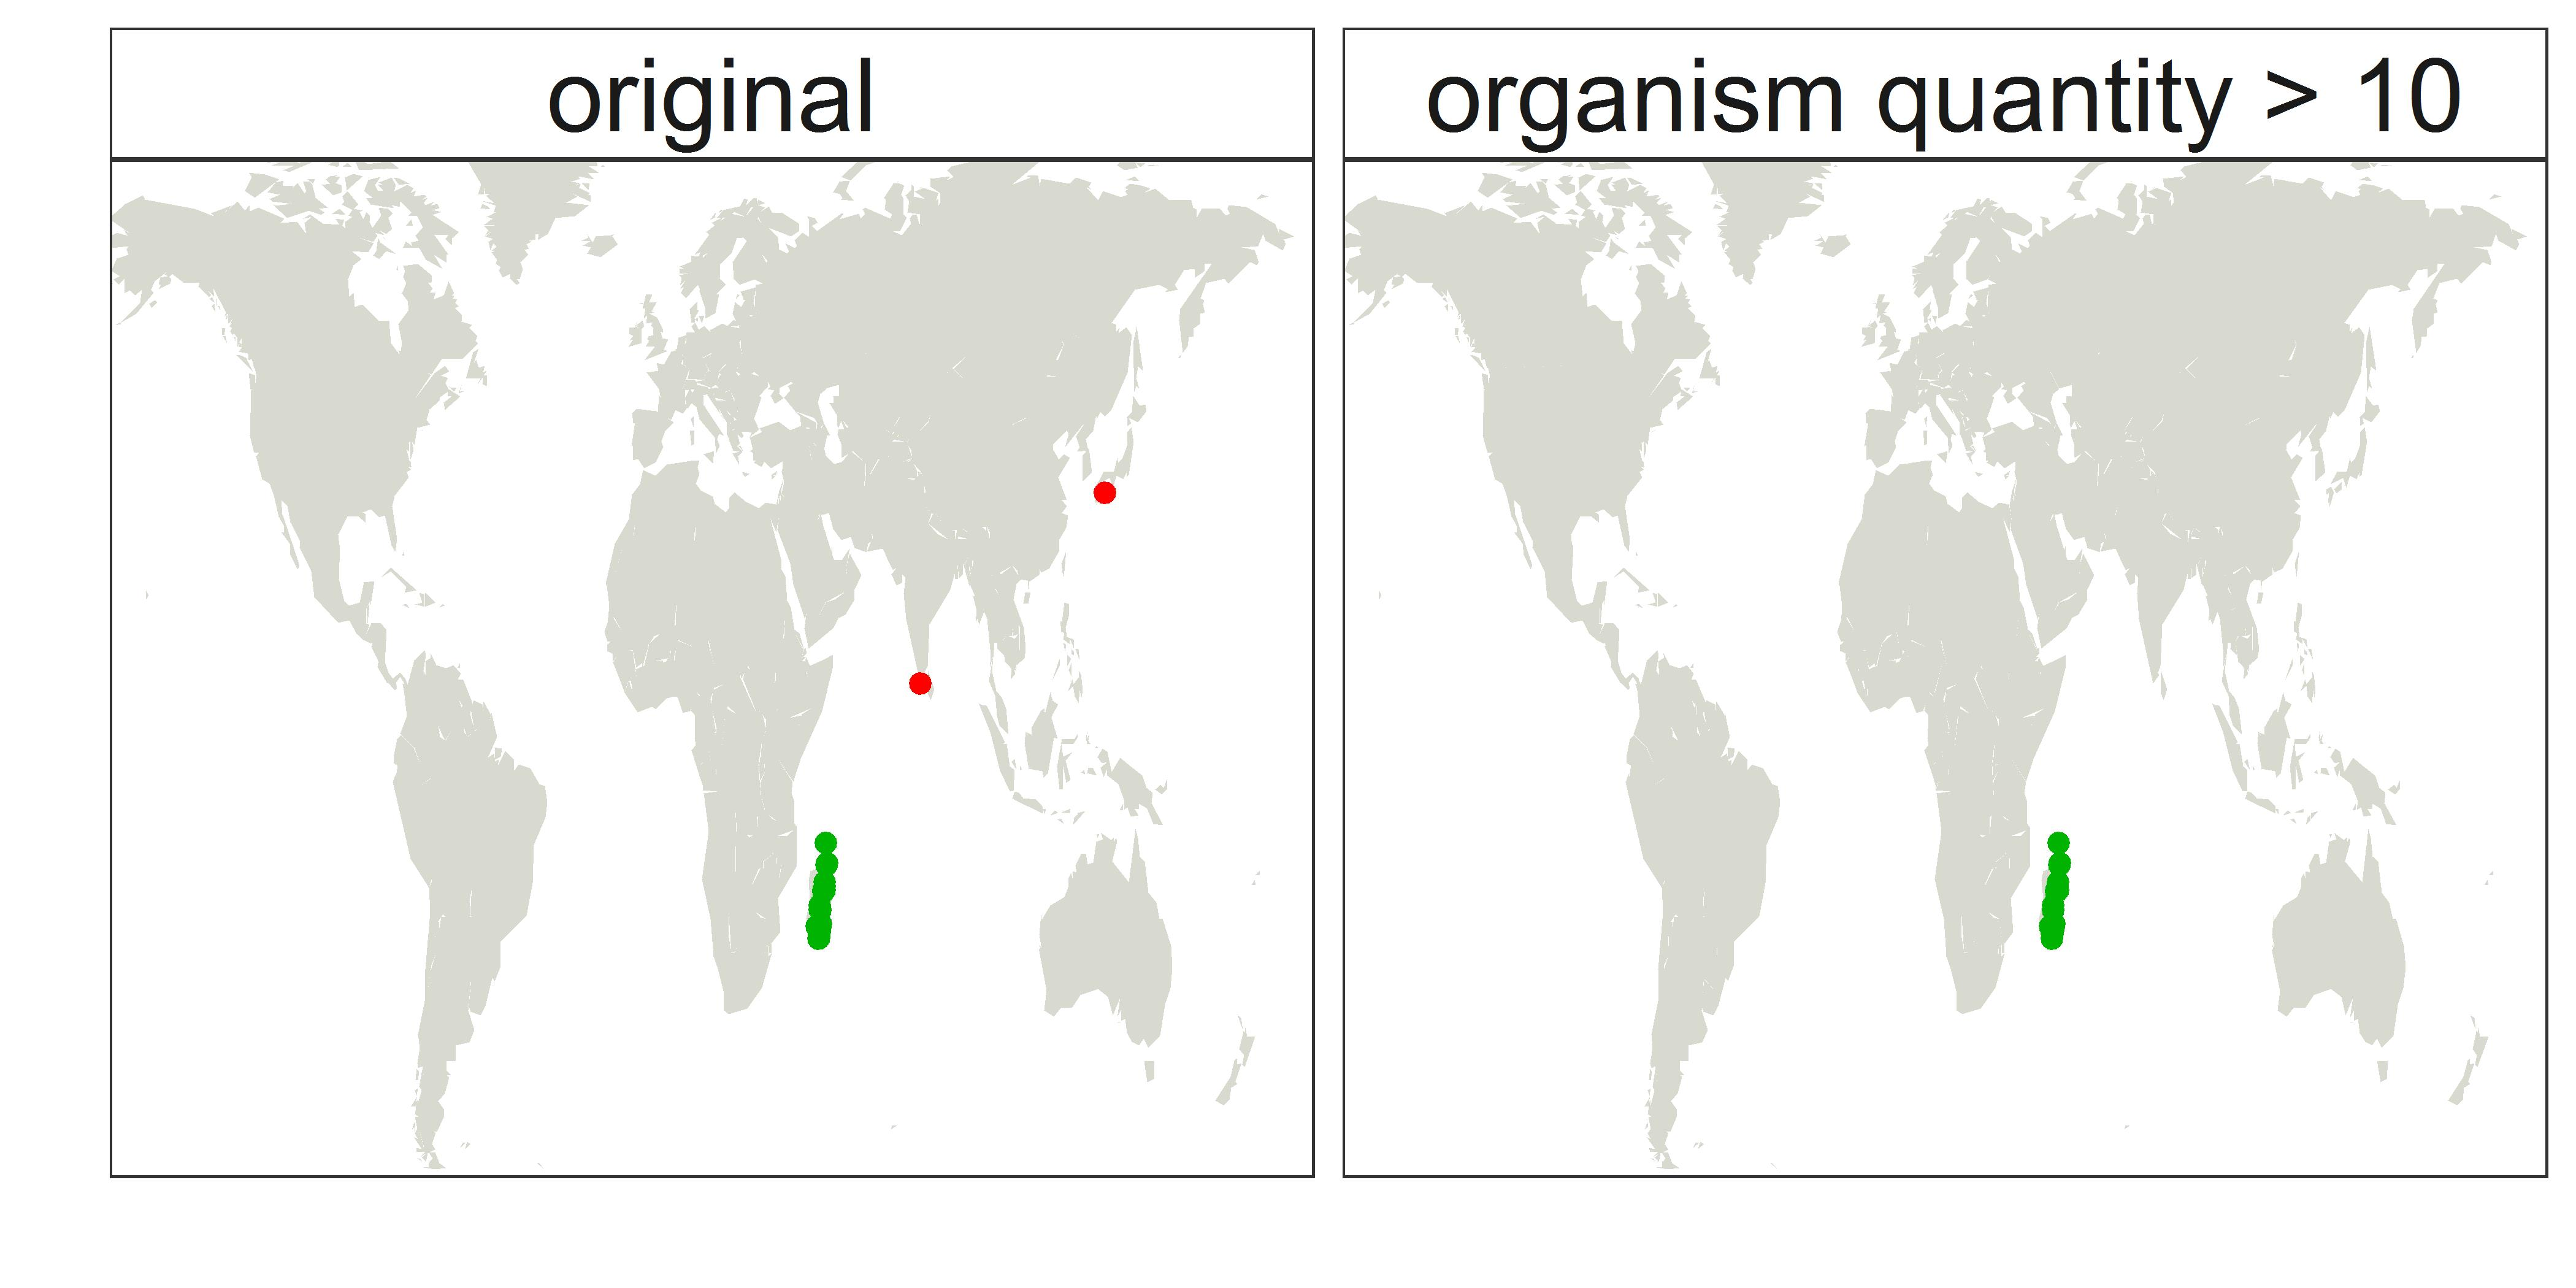
\includegraphics{/post/2020-01-08-metagenomics-occurrences-on-gbif_files/comparison_plot_7357804.jpg}

\hypertarget{frog-native-to-nepal}{%
\subsubsection{Frog (native to Nepal)}\label{frog-native-to-nepal}}

\begin{itemize}
\tightlist
\item
  link to
  \href{https://www.gbif.org/occurrence/map?taxon_key=2430314}{gbif map}
\end{itemize}

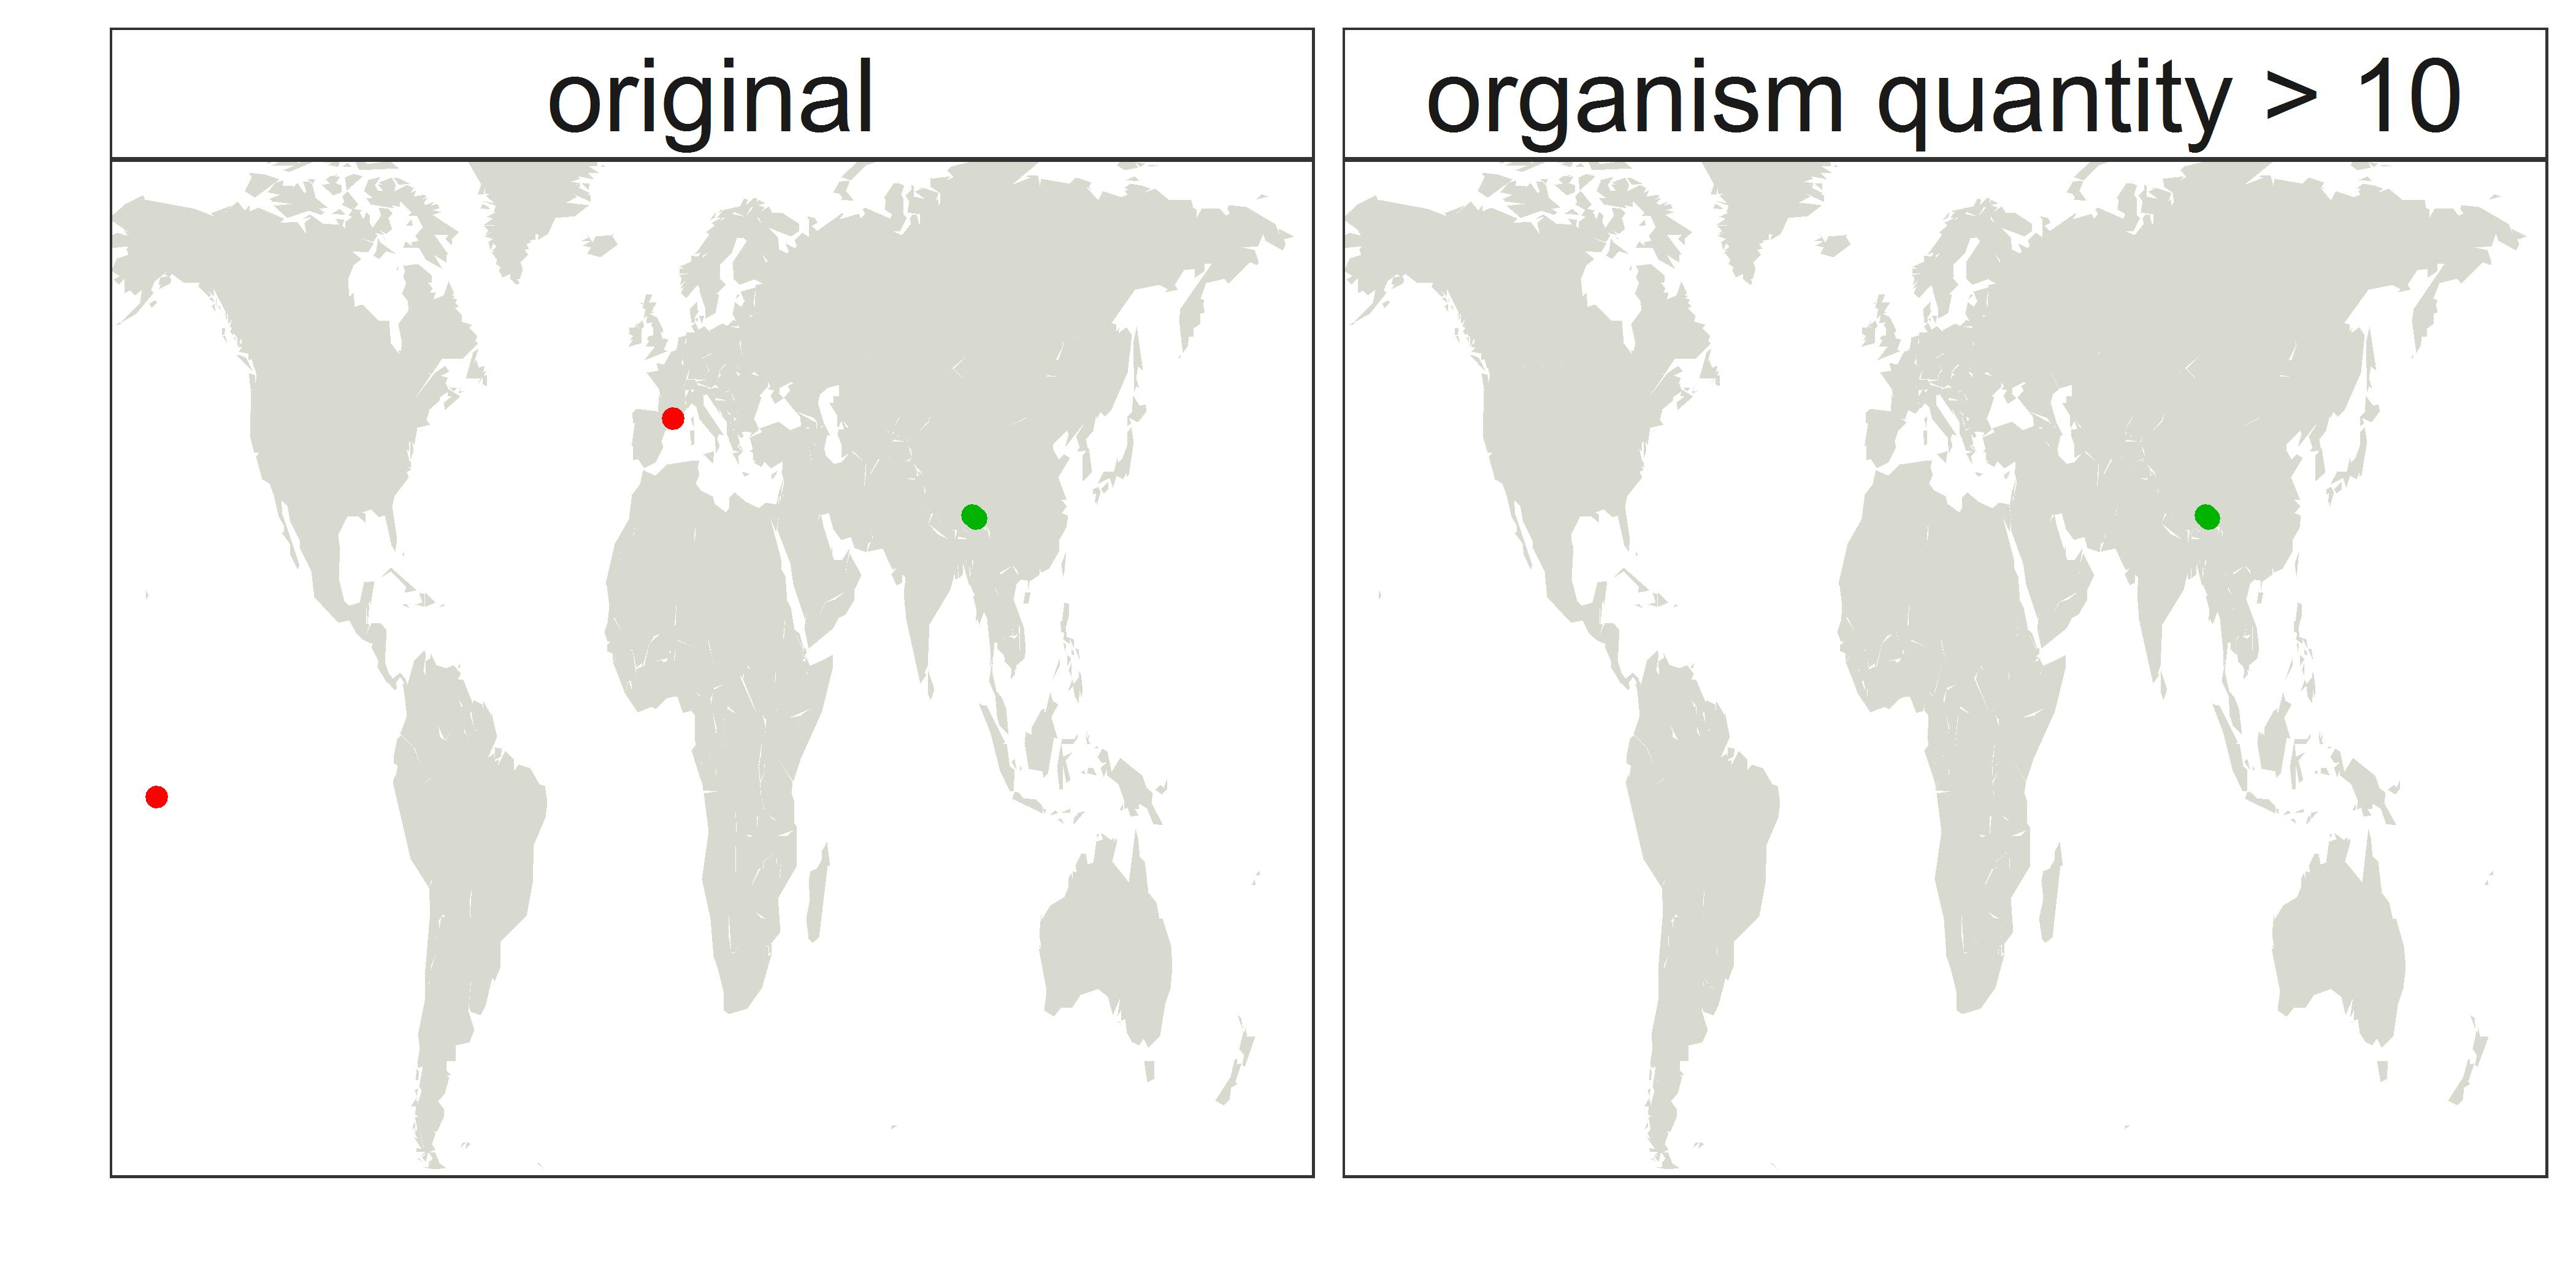
\includegraphics{/post/2020-01-08-metagenomics-occurrences-on-gbif_files/comparison_plot_2430314.jpg}

\hypertarget{turtle}{%
\subsubsection{Turtle}\label{turtle}}

\begin{itemize}
\tightlist
\item
  link to
  \href{https://www.gbif.org/occurrence/map?taxon_key=2443212}{gbif map}
\item
  The remaining point in Indoneisa is from Naturgucker (citizen science)
\end{itemize}

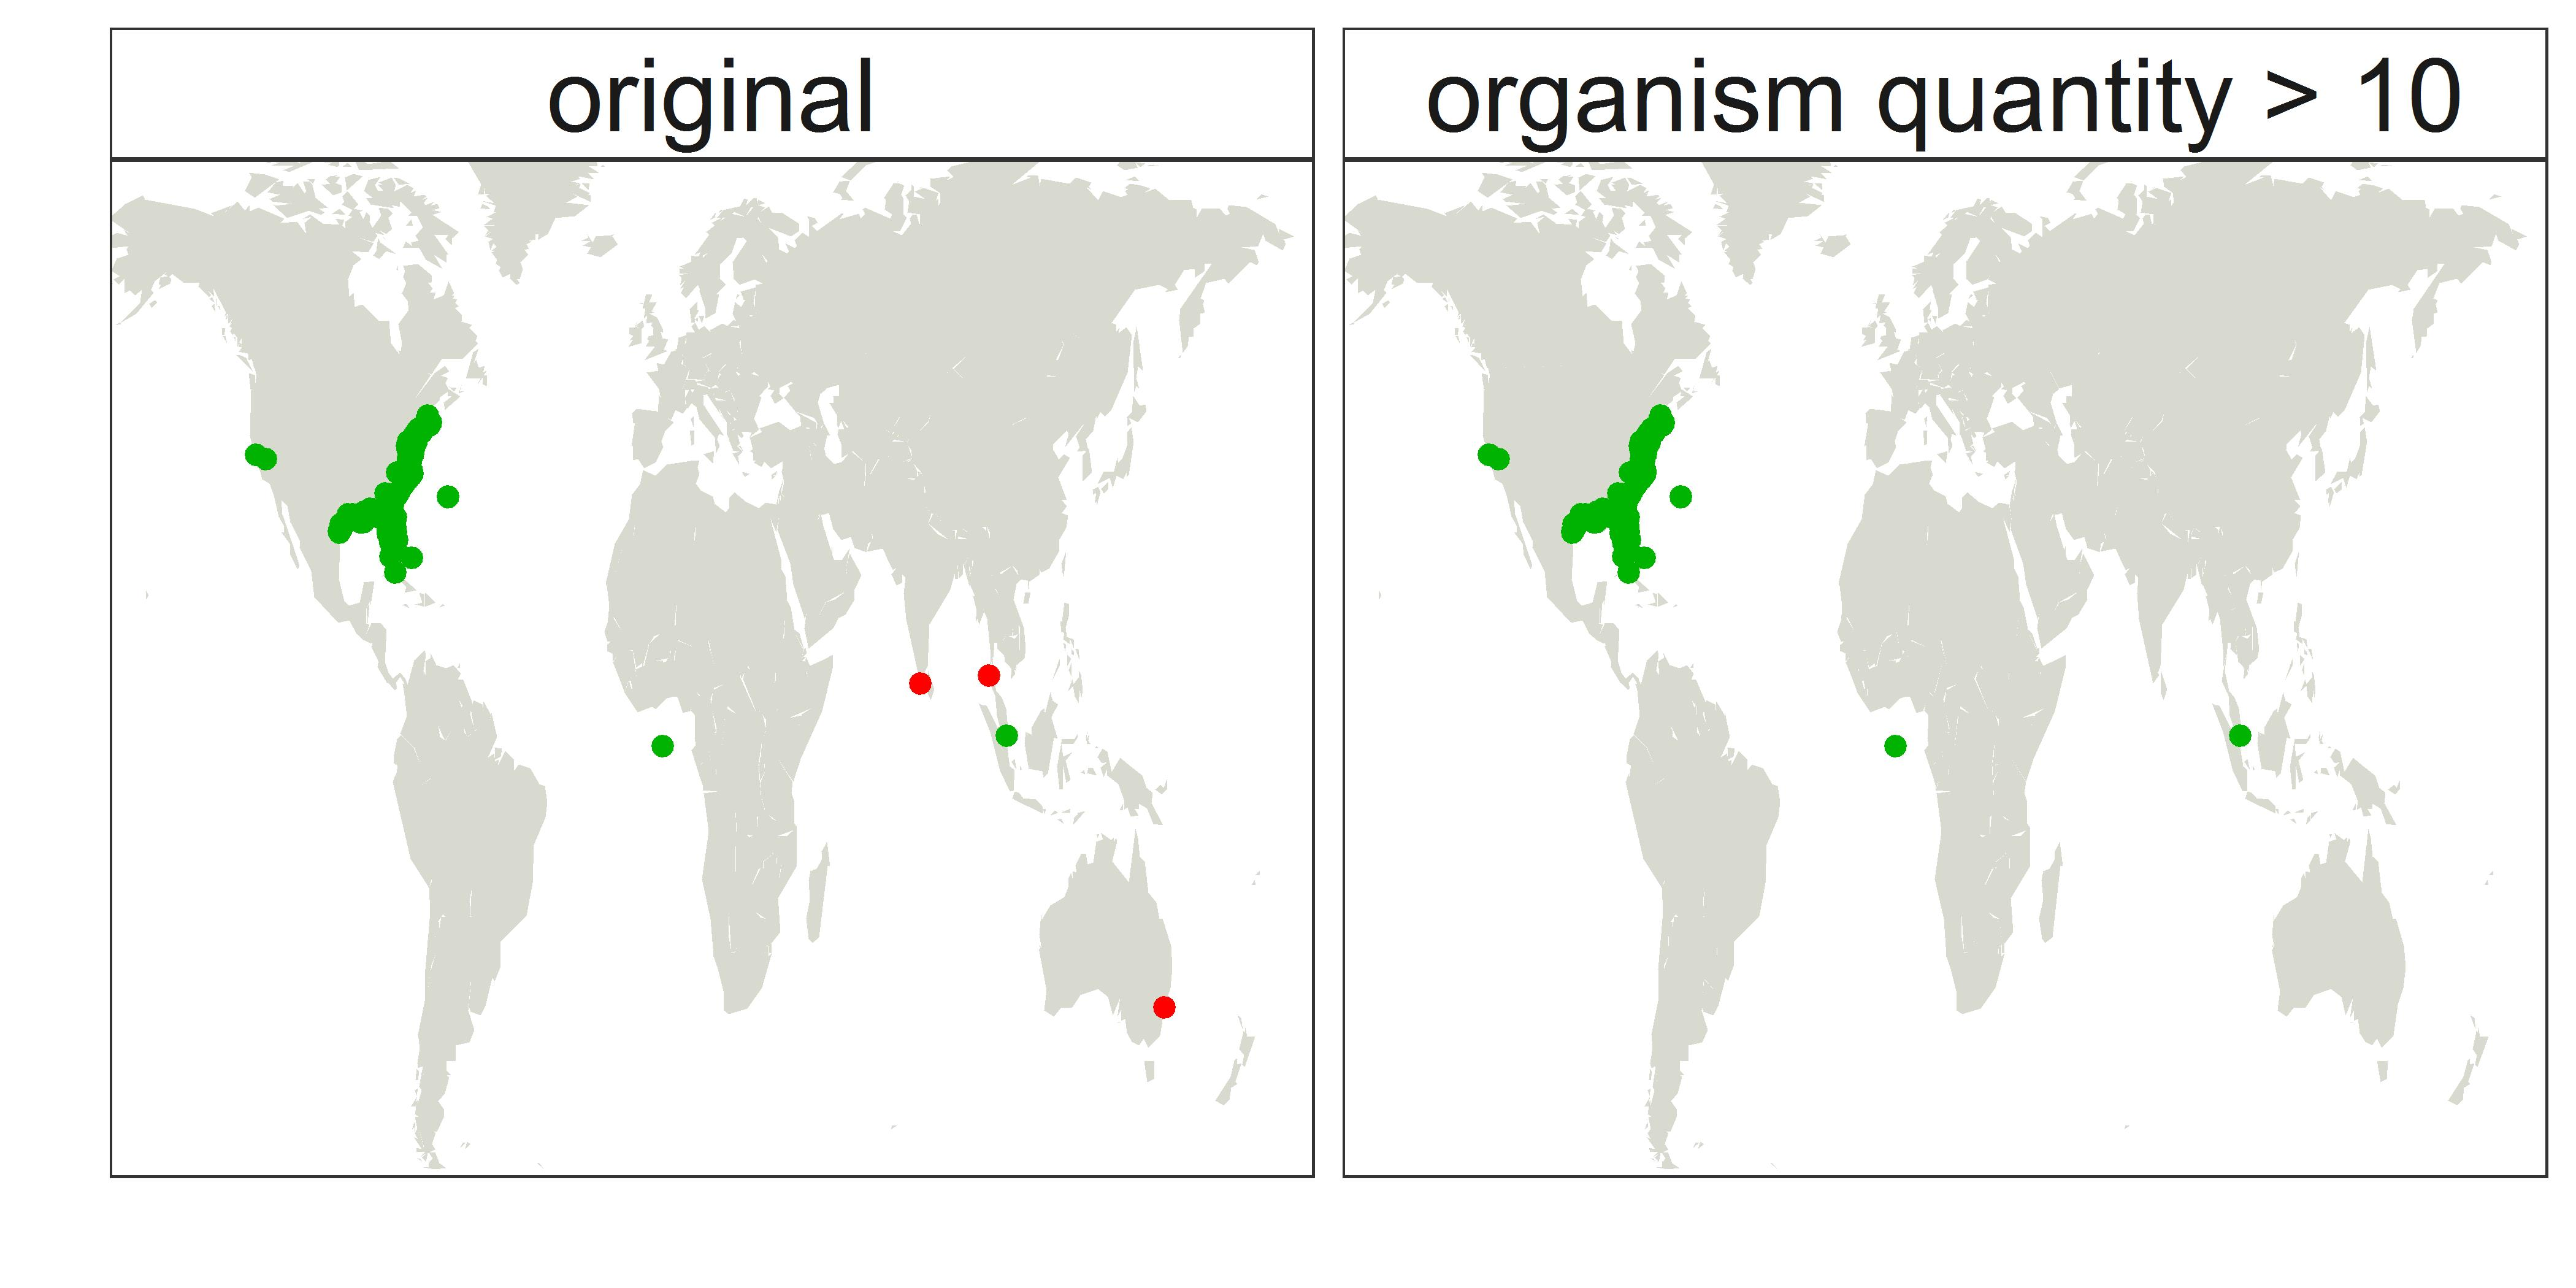
\includegraphics{/post/2020-01-08-metagenomics-occurrences-on-gbif_files/comparison_plot_2443212.jpg}

\hypertarget{vulture}{%
\subsubsection{Vulture}\label{vulture}}

\begin{itemize}
\tightlist
\item
  link to
  \href{https://www.gbif.org/occurrence/gallery?taxon_key=5229165}{gbif
  map}
\item
  Difficult to tell if {metagenomics points} are legitmate.
\item
  One of only two bird records (at rank species) in MGnify. The other is
  the kiwi bird shown above.
\end{itemize}

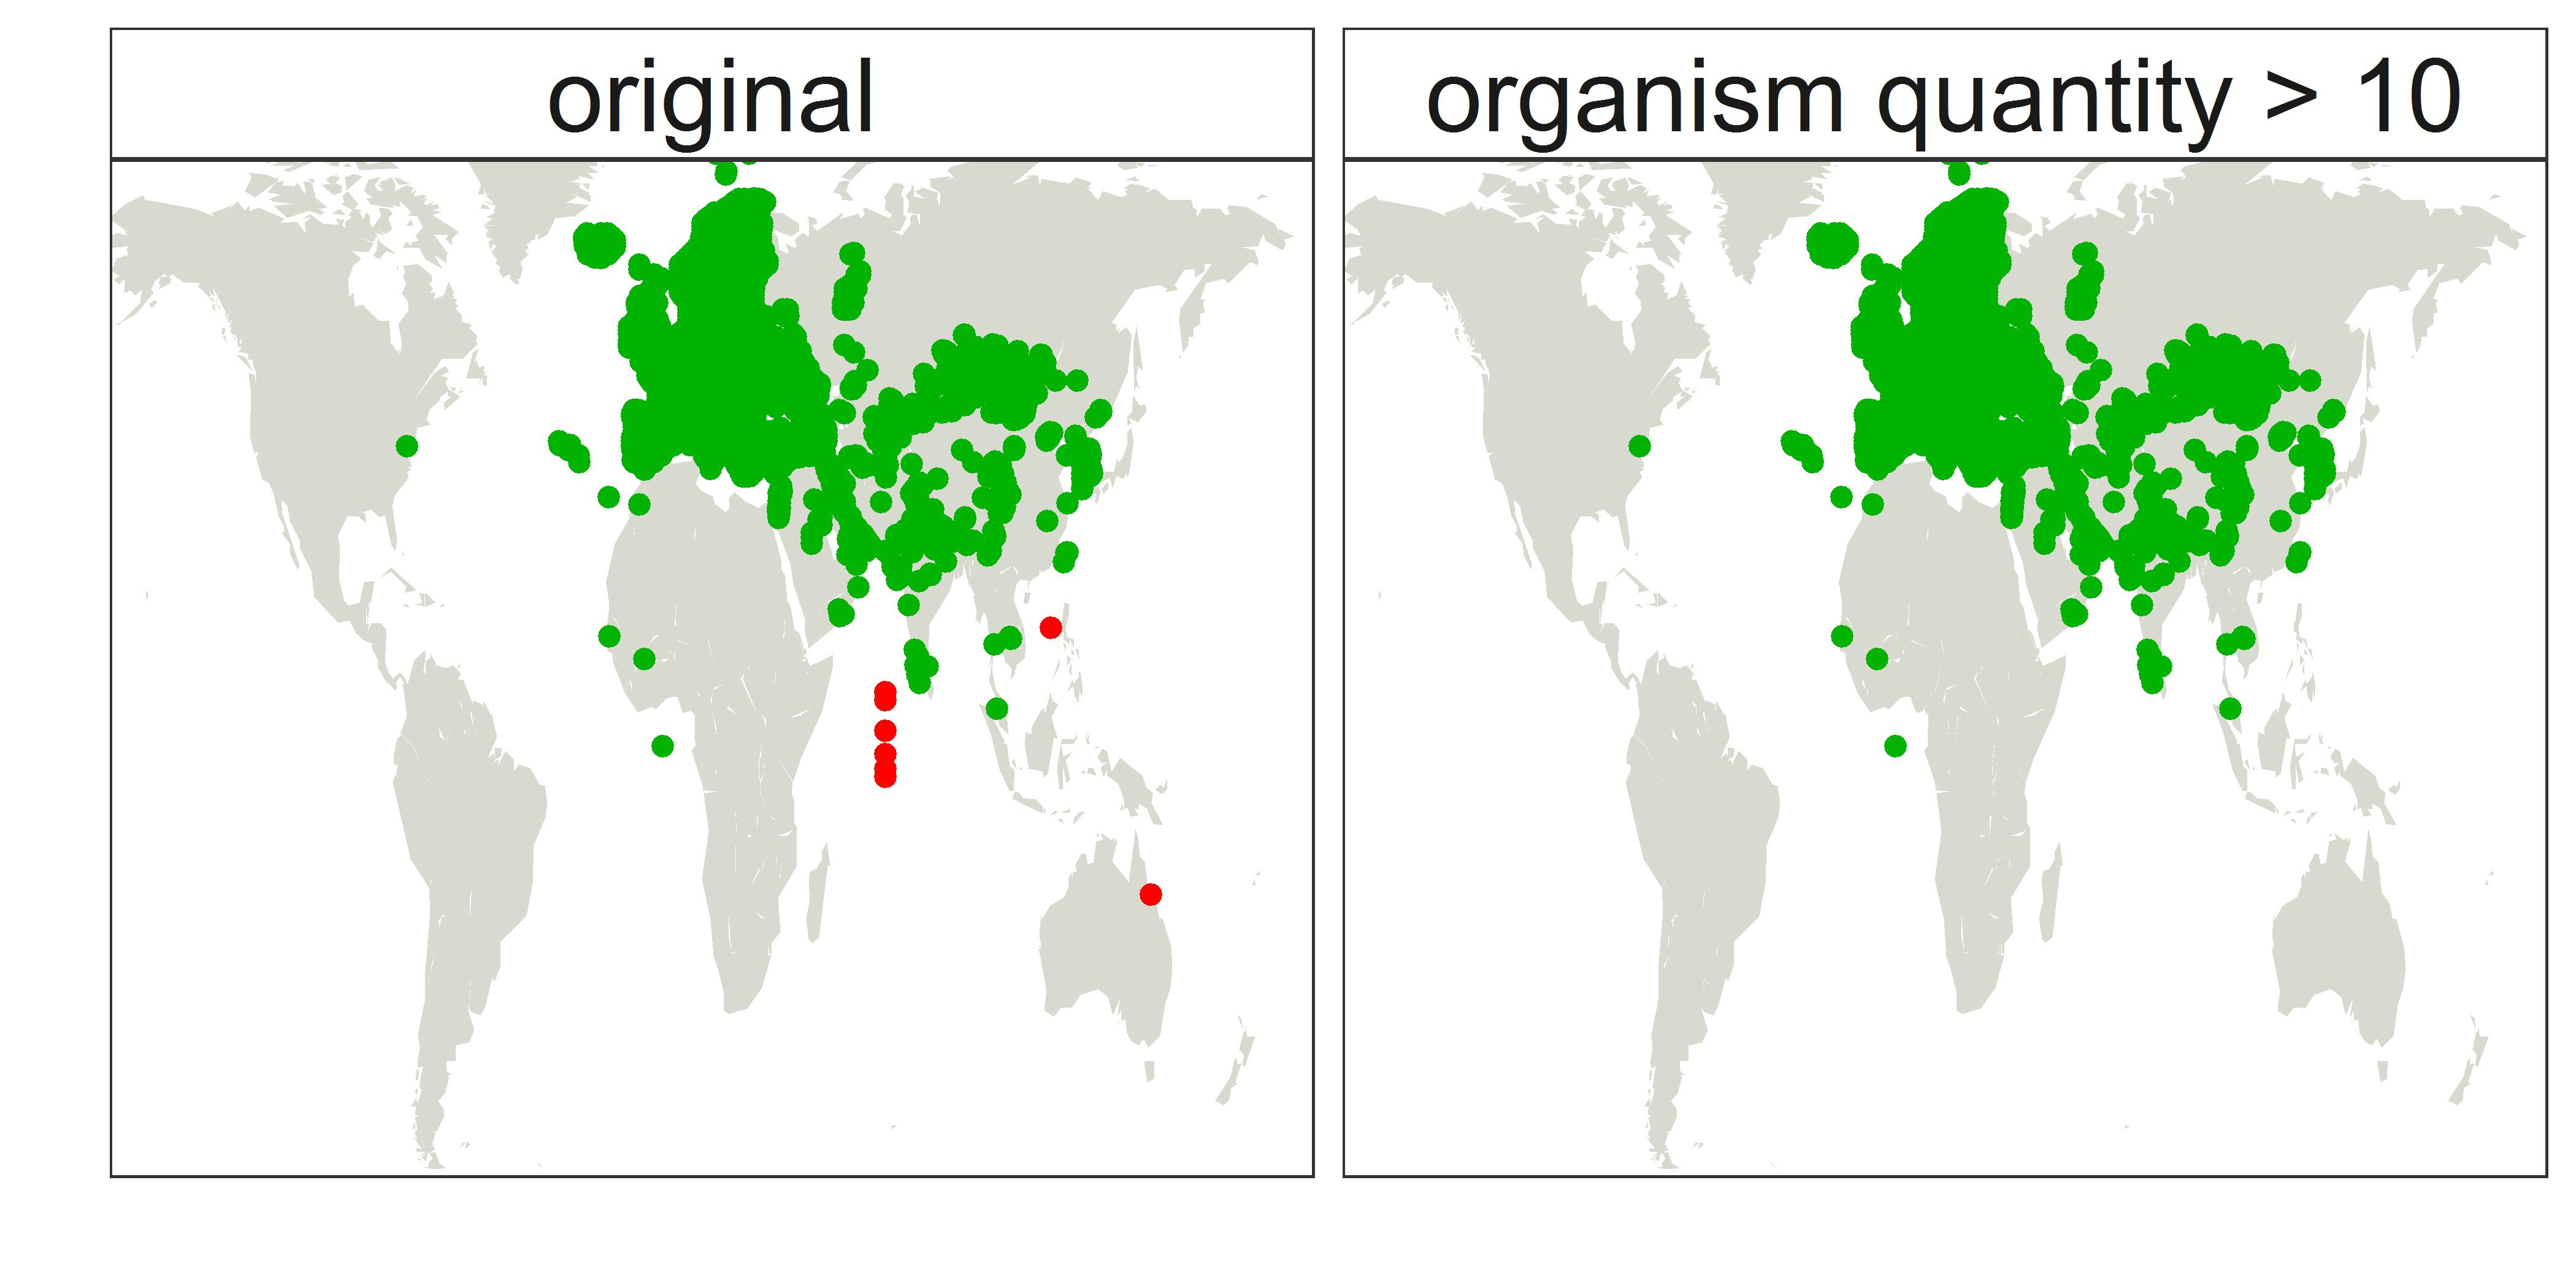
\includegraphics{/post/2020-01-08-metagenomics-occurrences-on-gbif_files/comparison_plot_5229165.jpg}

\hypertarget{white-rhinoceros}{%
\subsubsection{White rhinoceros}\label{white-rhinoceros}}

\begin{itemize}
\tightlist
\item
  link to
  \href{https://www.gbif.org/occurrence/map?taxon_key=2440880}{gbif map}
\item
  The
  \href{https://www.gbif.org/occurrence/search?has_coordinate=true\&taxon_key=2440880\&advanced=1\&geometry=POLYGON((-112.41211\%2025.48828,-73.91602\%2025.48828,-73.91602\%2045.17578,-112.41211\%2045.17578,-112.41211\%2025.48828))}{two
  points} in the USA are from sound recording datasets or taken from
  zoos.
\end{itemize}

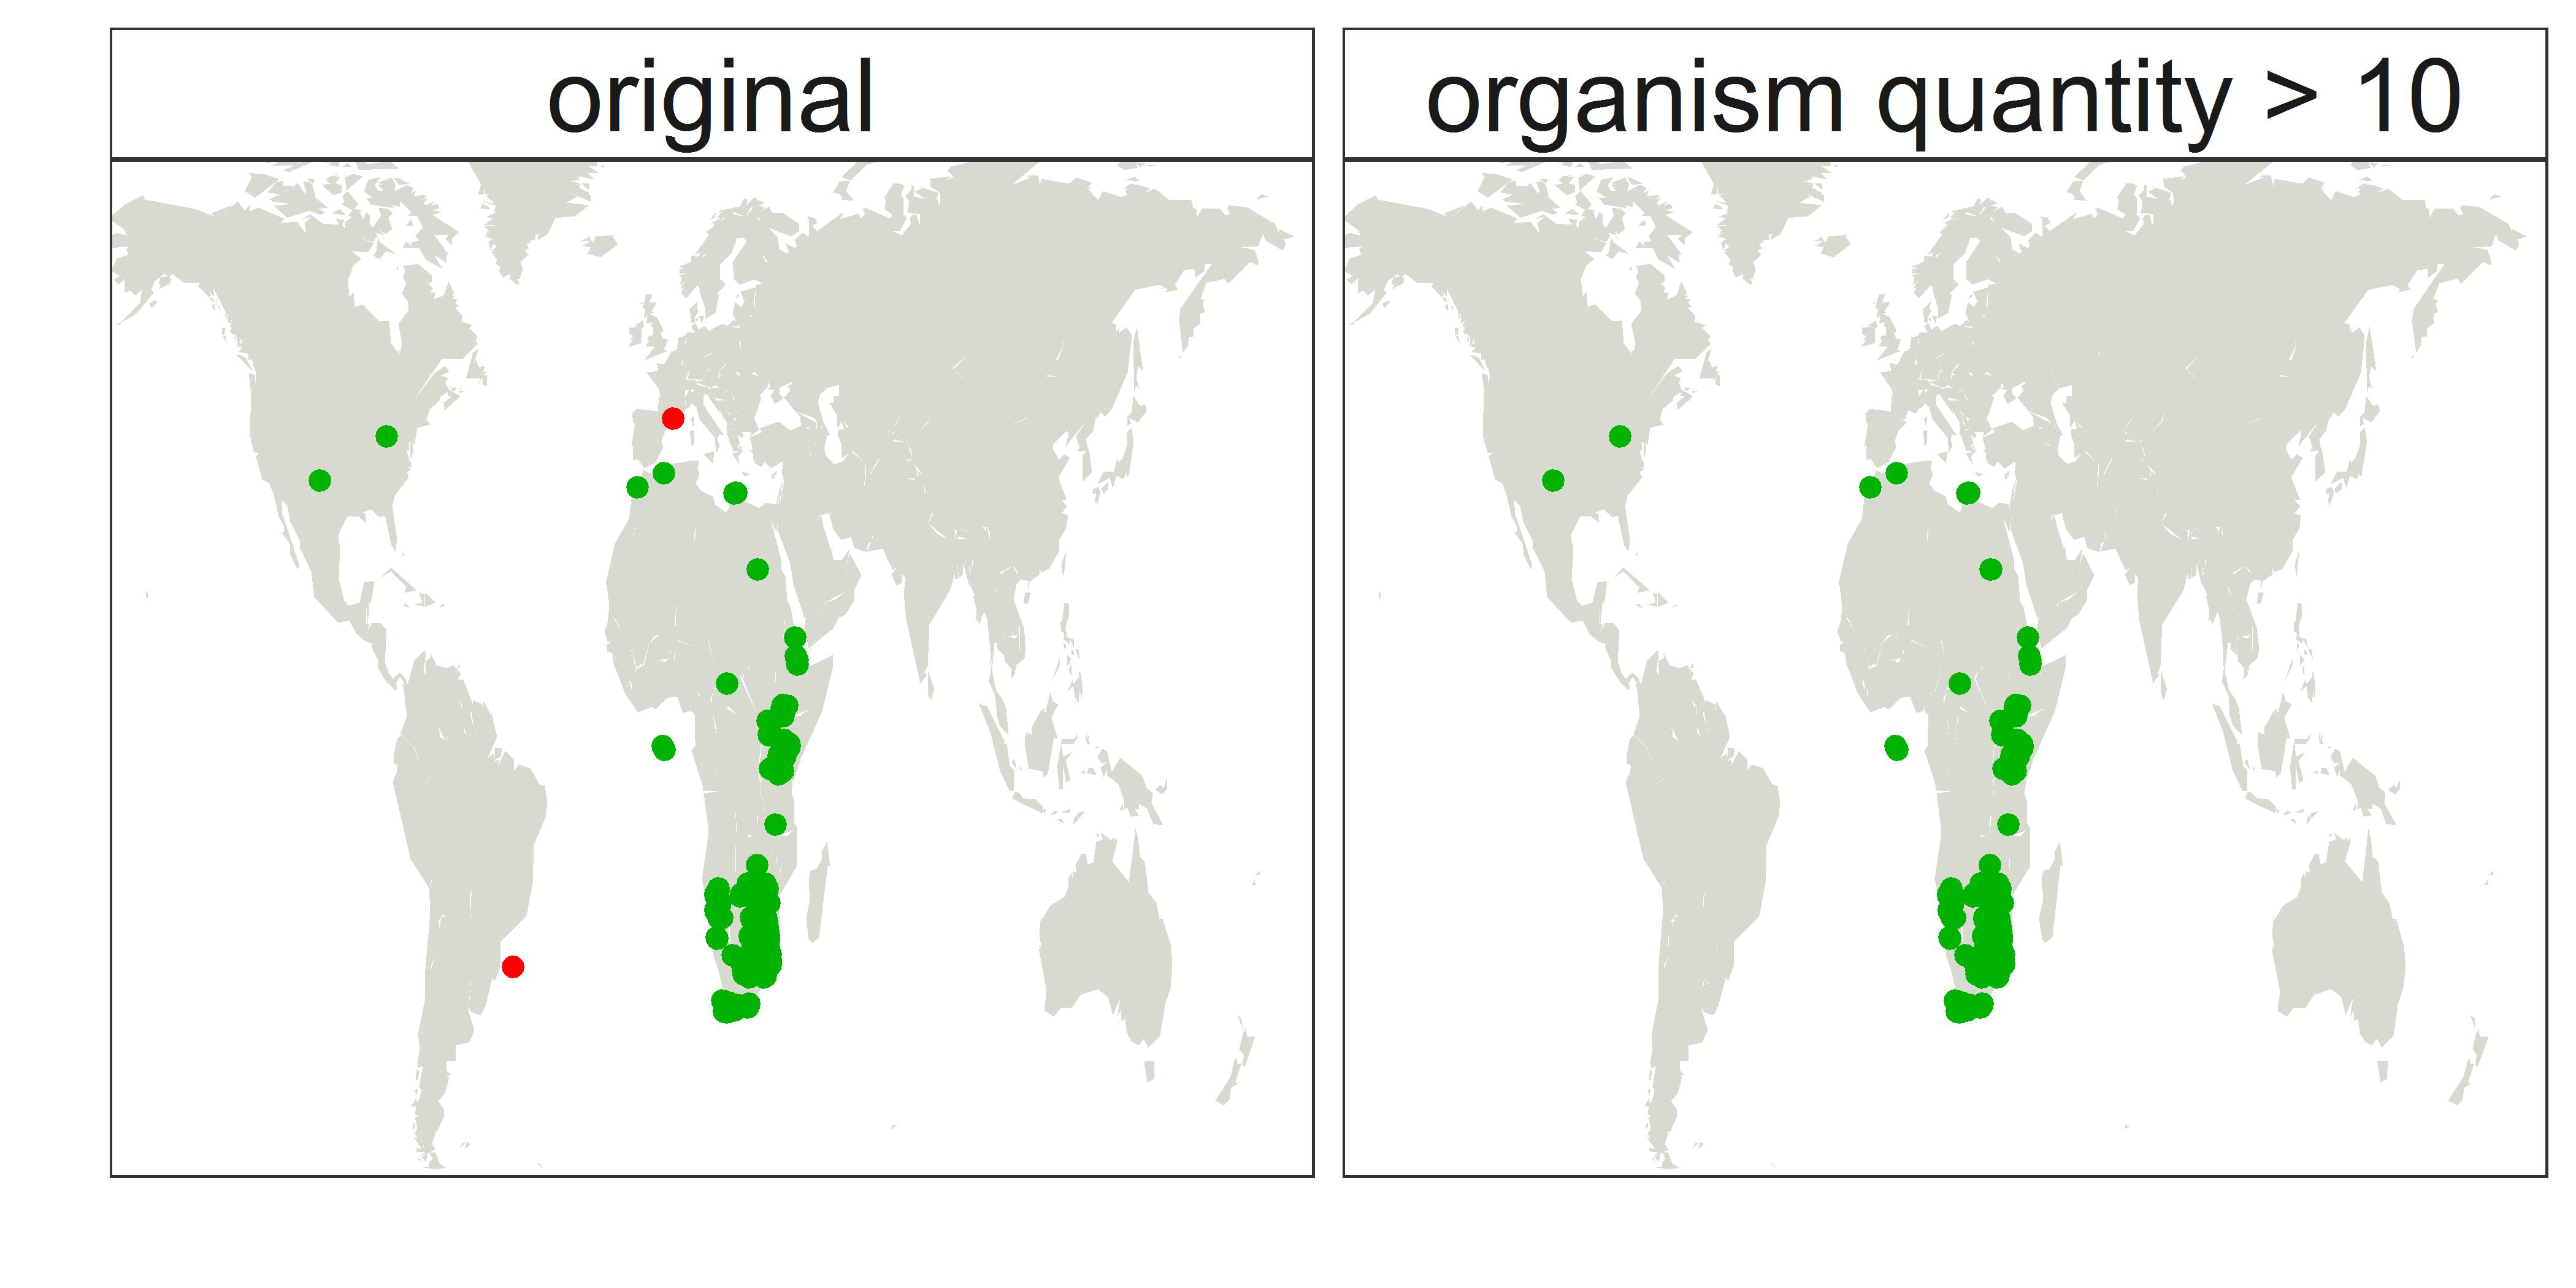
\includegraphics{/post/2020-01-08-metagenomics-occurrences-on-gbif_files/comparison_plot_2440880.jpg}

\hypertarget{bison}{%
\subsubsection{Bison}\label{bison}}

\begin{itemize}
\tightlist
\item
  link to
  \href{https://www.gbif.org/occurrence/map?taxon_key=2441176}{gbif map}
\item
  Some of the points in Europe are from Naturgurker (citizen science).
\item
  Record in Africa from
  \href{https://www.gbif.org/occurrence/1064936544}{farm}
\item
  Record in India seems like from
  \href{https://www.gbif.org/occurrence/1065408095}{museum}
\end{itemize}

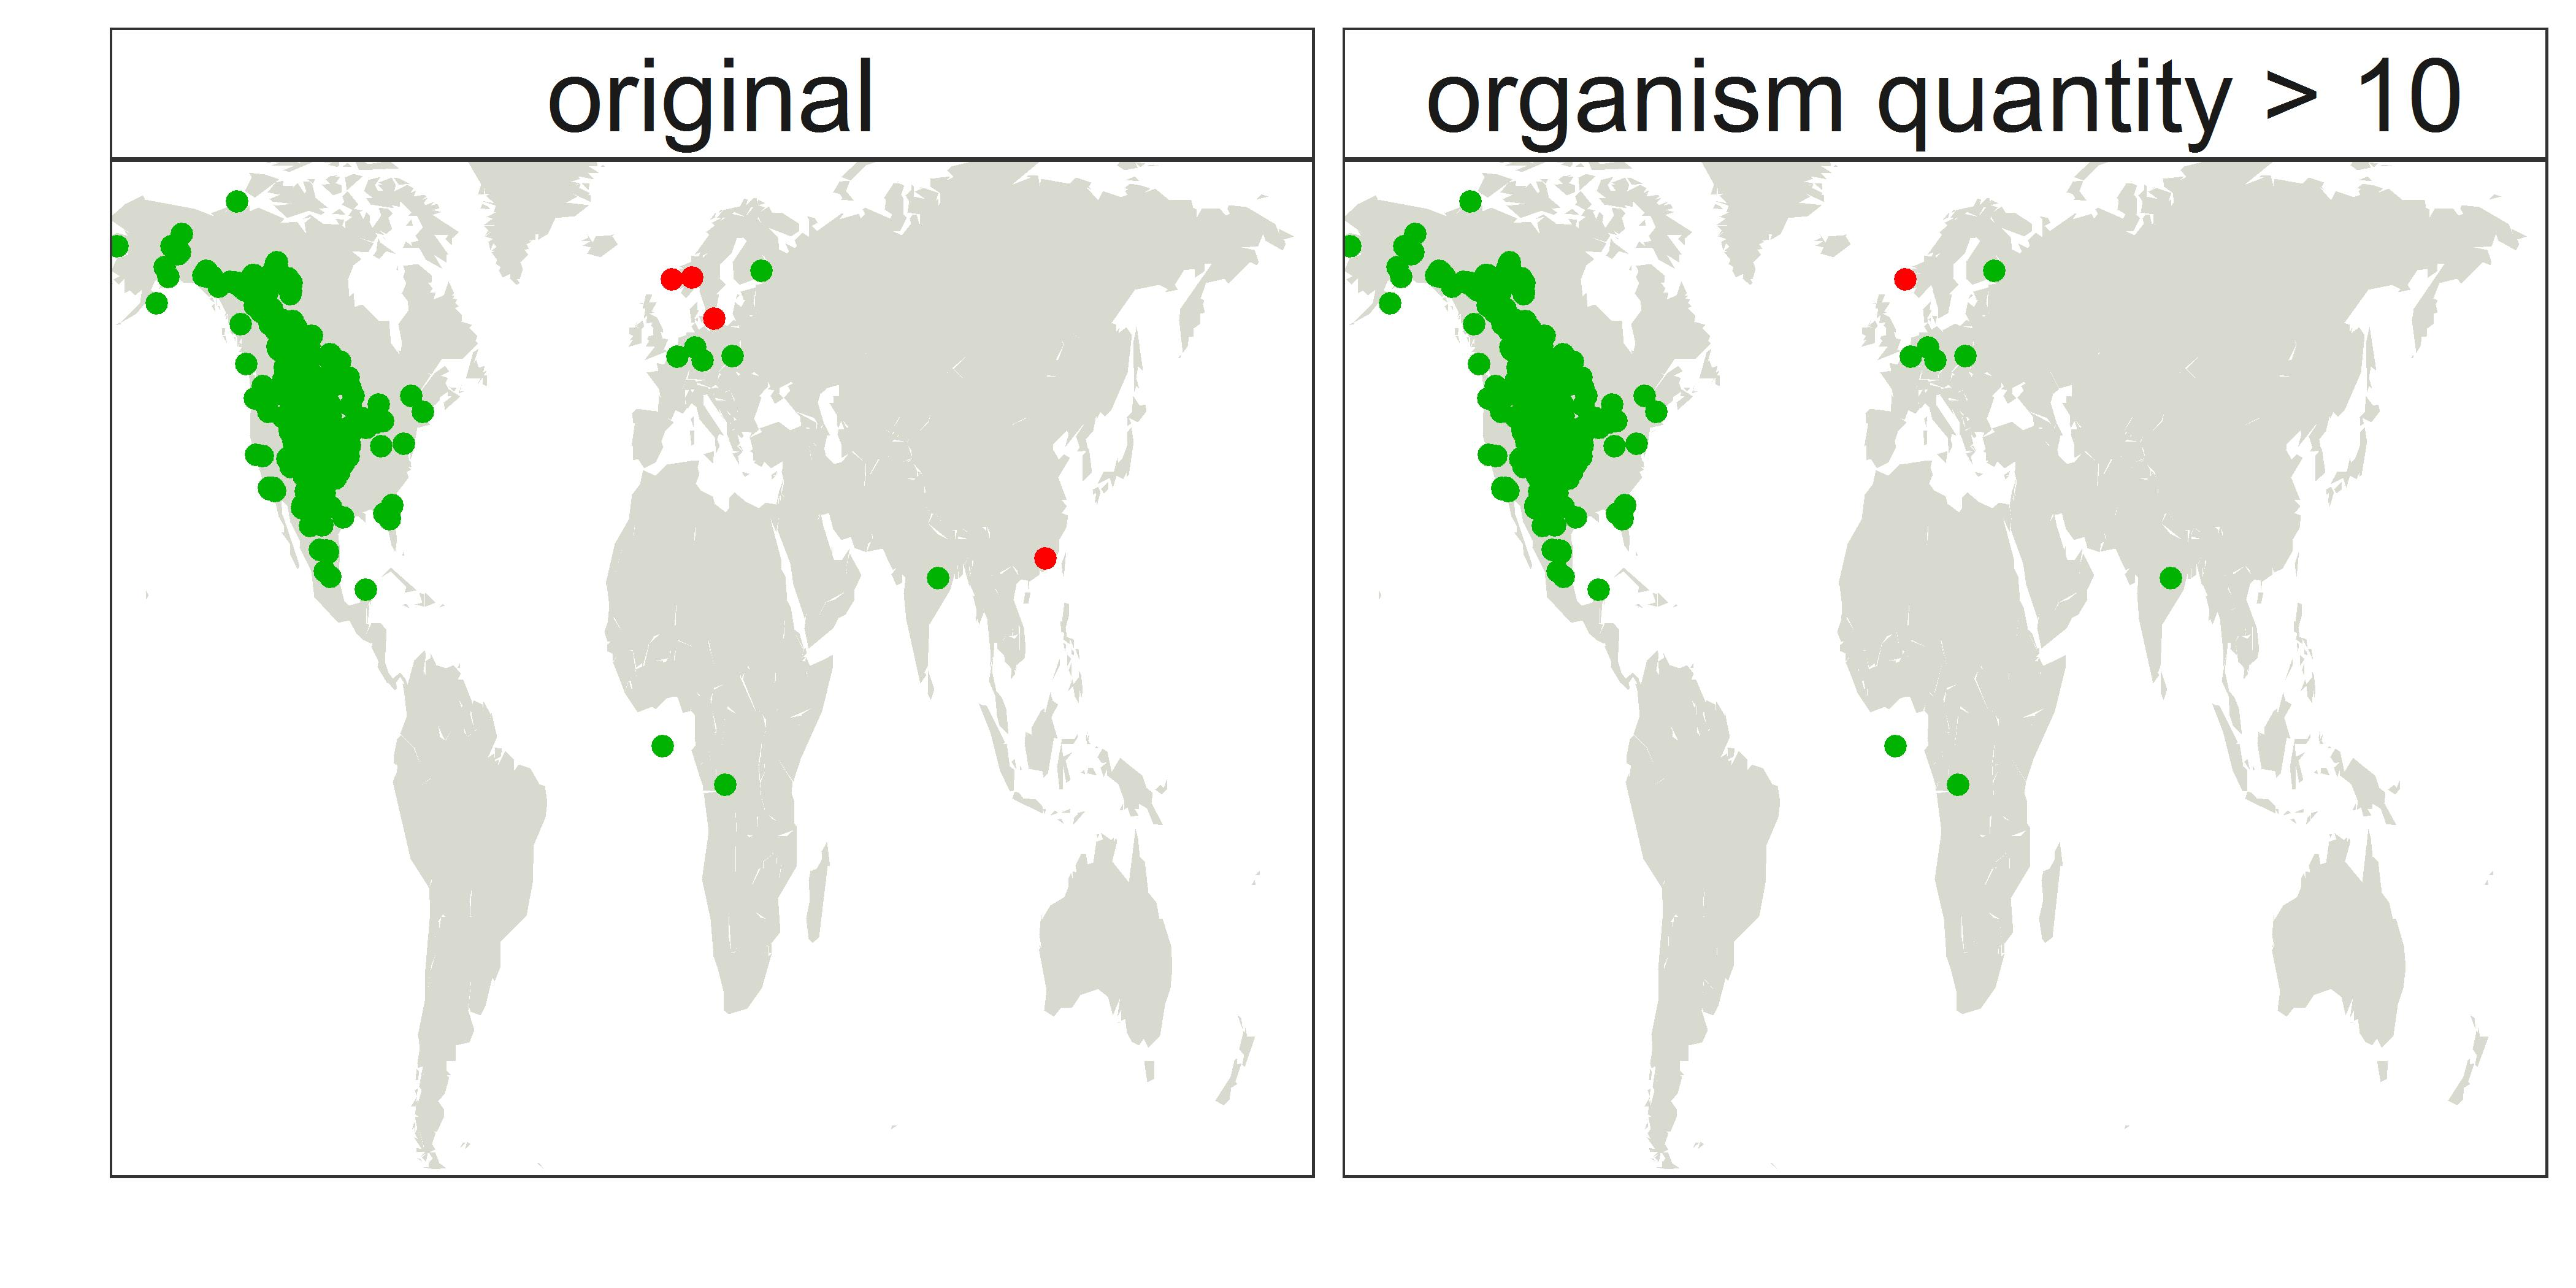
\includegraphics{/post/2020-01-08-metagenomics-occurrences-on-gbif_files/comparison_plot_2441176.jpg}

\hypertarget{beetle}{%
\subsubsection{Beetle}\label{beetle}}

\begin{itemize}
\tightlist
\item
  link to
  \href{https://www.gbif.org/occurrence/map?taxon_key=7661194}{gbif map}
\item
  {Metagenomic point} in Europe seems very unlikely.
\end{itemize}

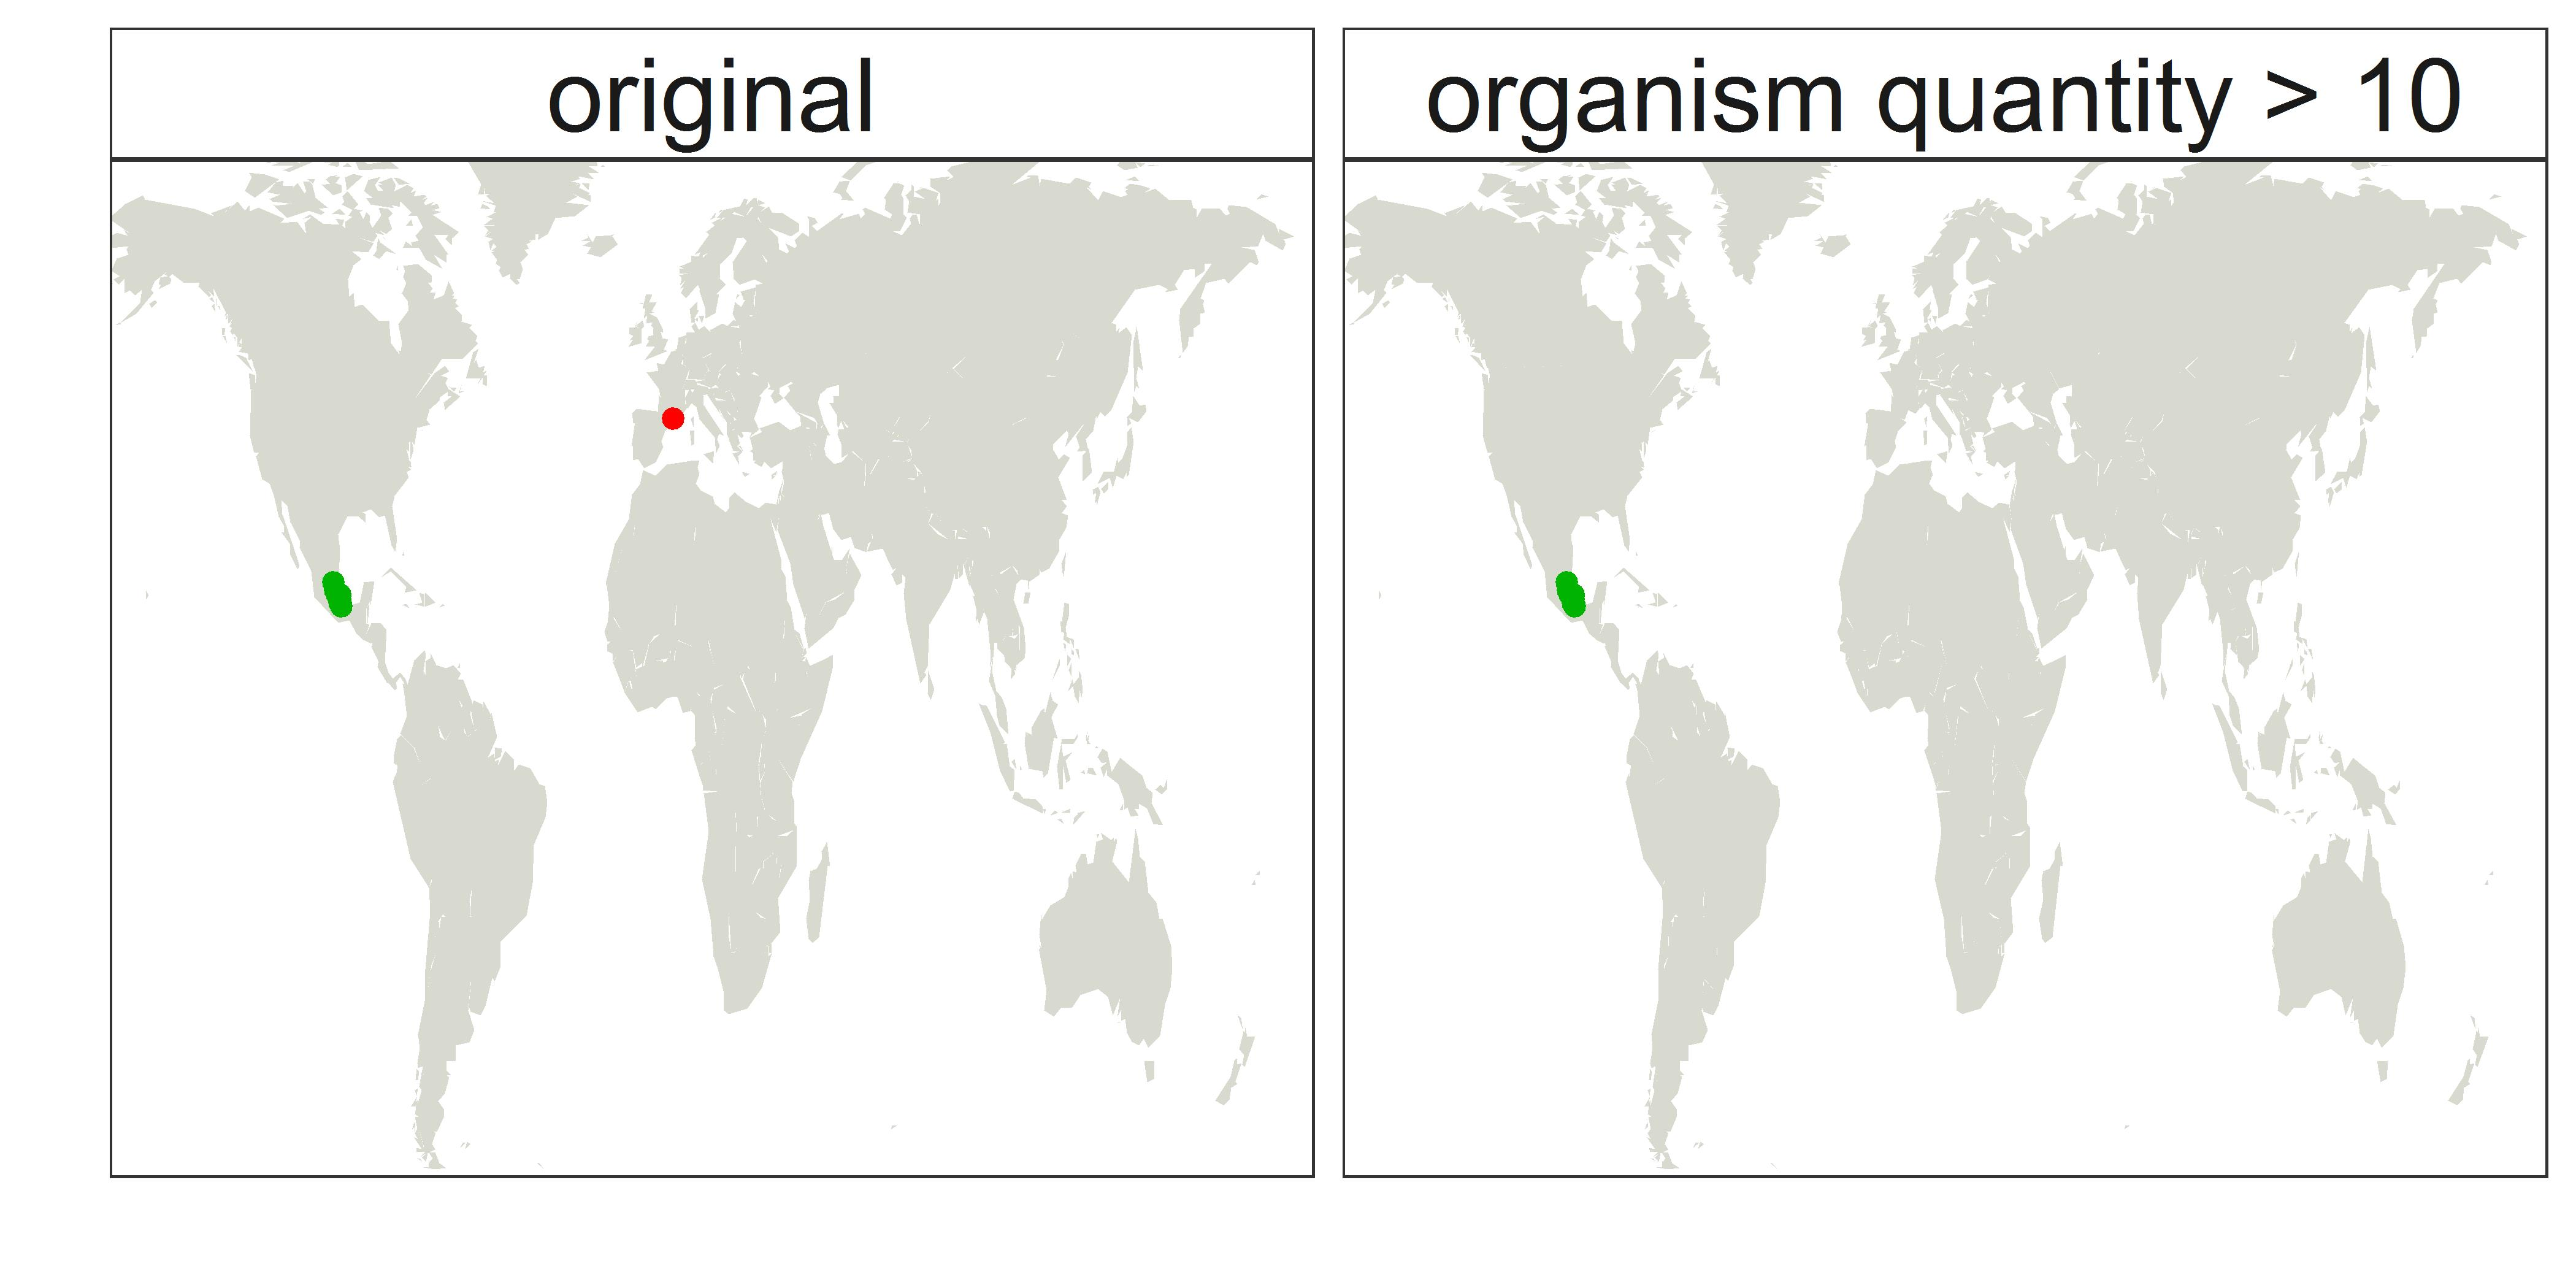
\includegraphics{/post/2020-01-08-metagenomics-occurrences-on-gbif_files/comparison_plot_7661194.jpg}

\hypertarget{toad}{%
\subsubsection{Toad}\label{toad}}

\begin{itemize}
\tightlist
\item
  link to
  \href{https://www.gbif.org/occurrence/map?taxon_key=2424395}{gbif map}
\item
  {metagenomics points} seem very unlikely
\end{itemize}

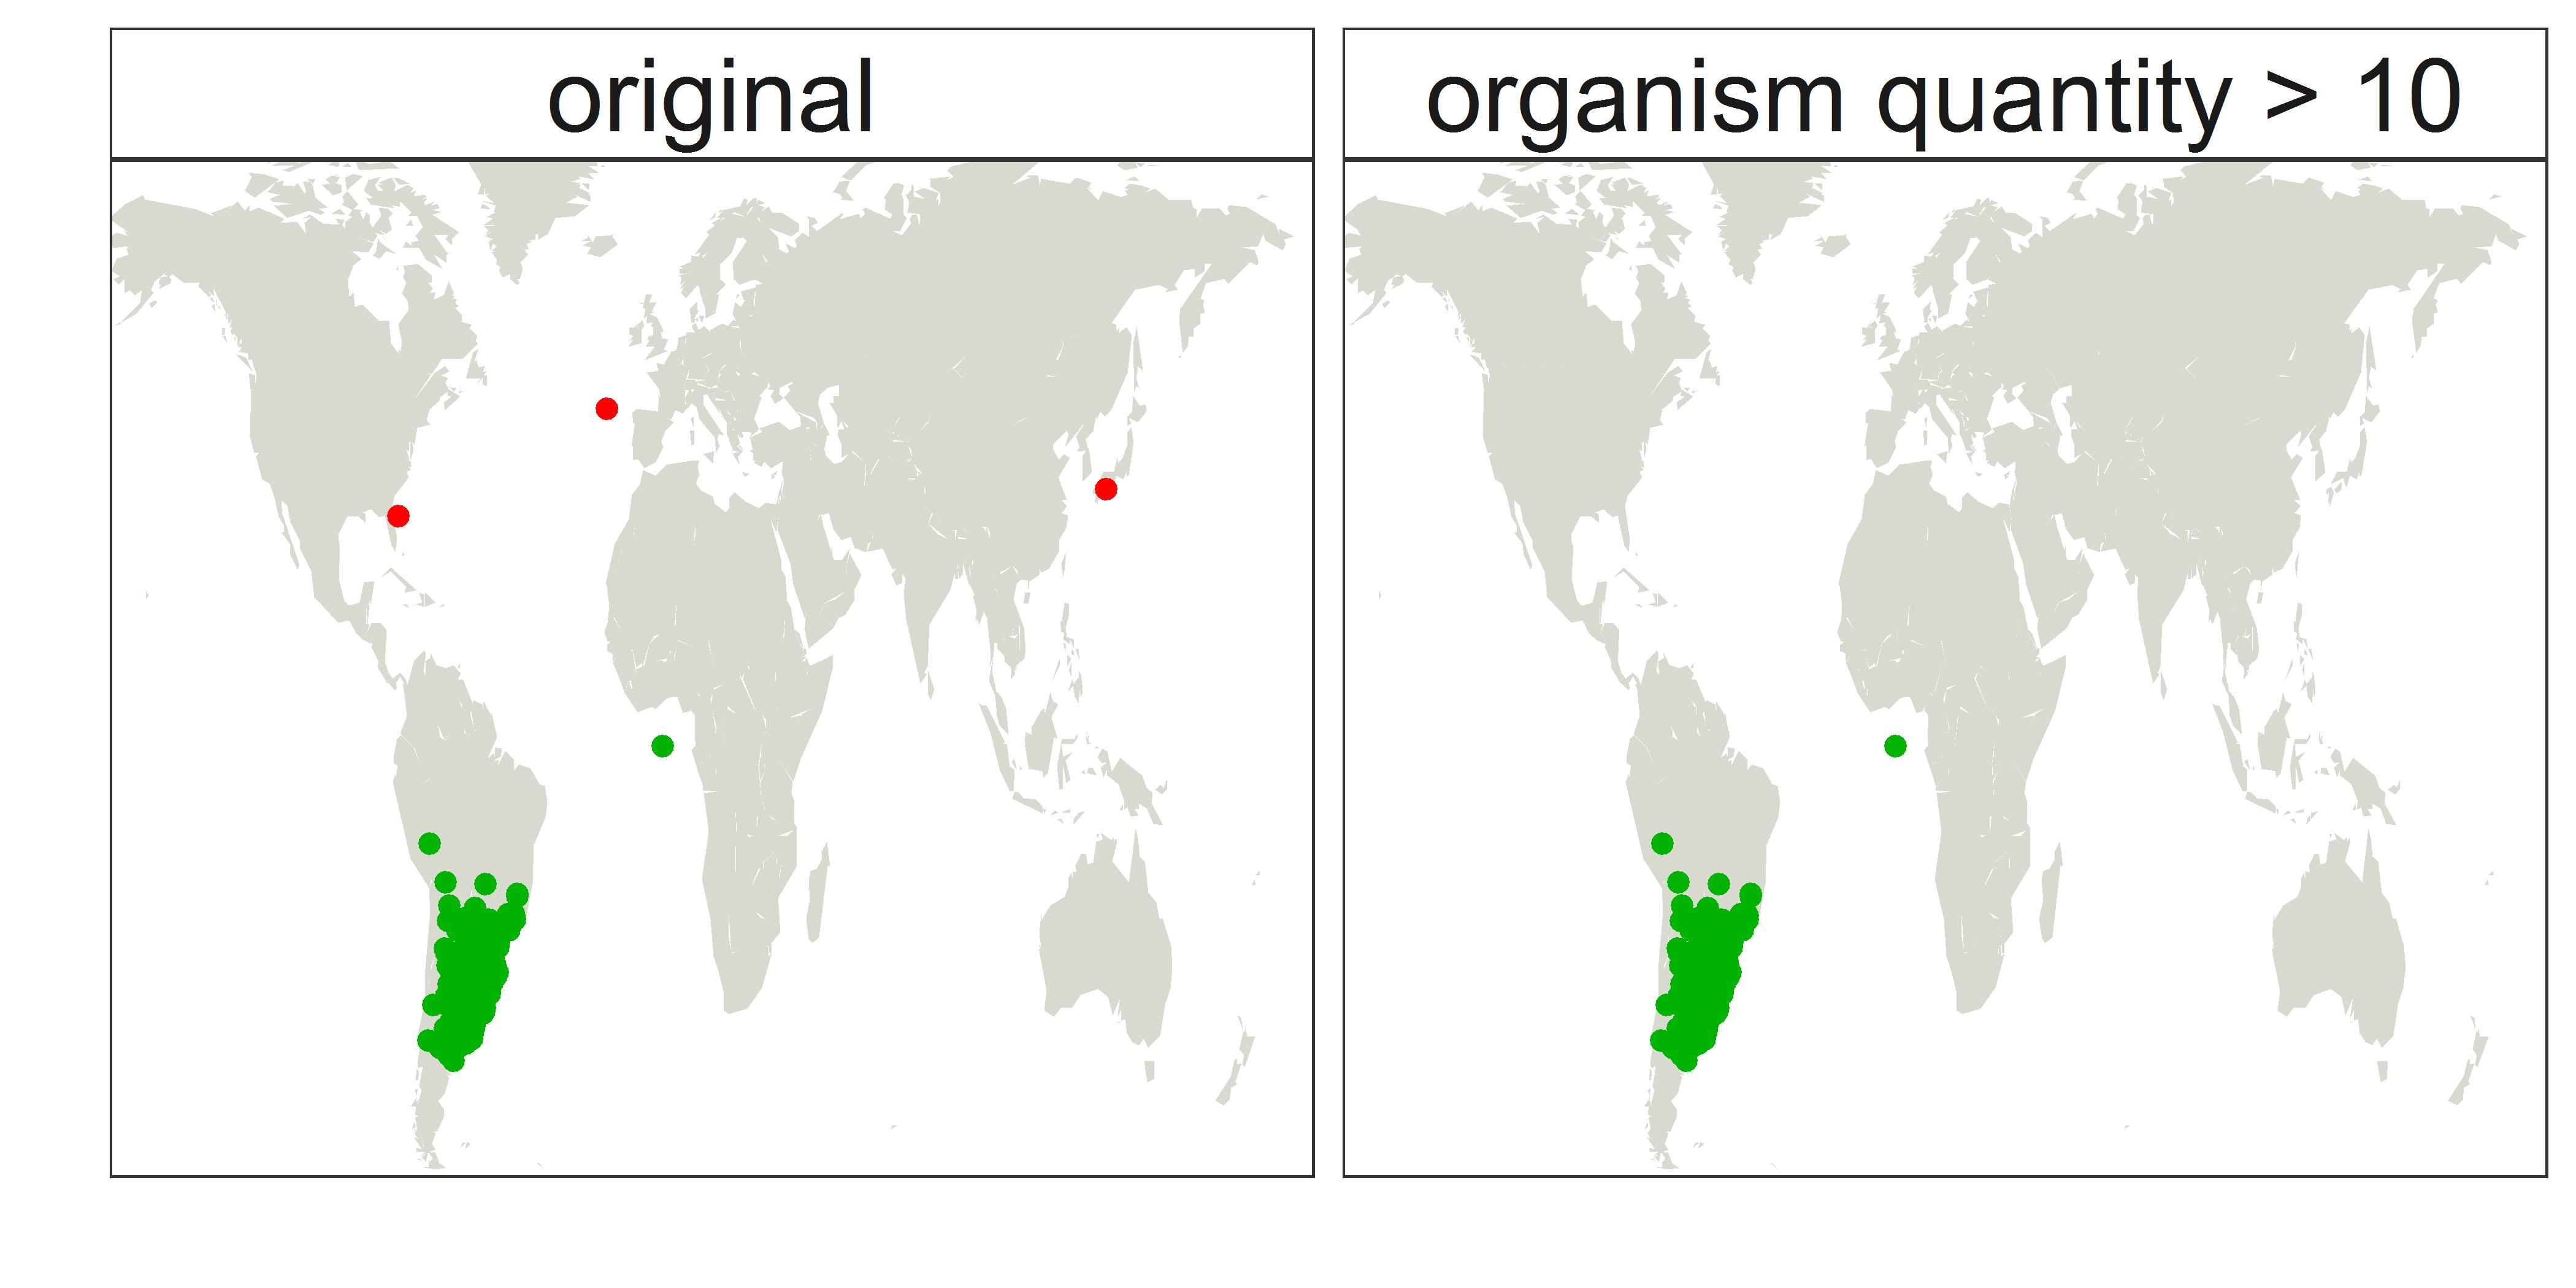
\includegraphics{/post/2020-01-08-metagenomics-occurrences-on-gbif_files/comparison_plot_2424395.jpg}

\hypertarget{fruit-piercing-insect}{%
\subsubsection{Fruit piercing insect}\label{fruit-piercing-insect}}

\begin{itemize}
\tightlist
\item
  link to
  \href{https://www.gbif.org/occurrence/map?taxon_key=1420595}{gbif map}
\item
  Only one dataset aside from MGnify has records of this species.
\end{itemize}

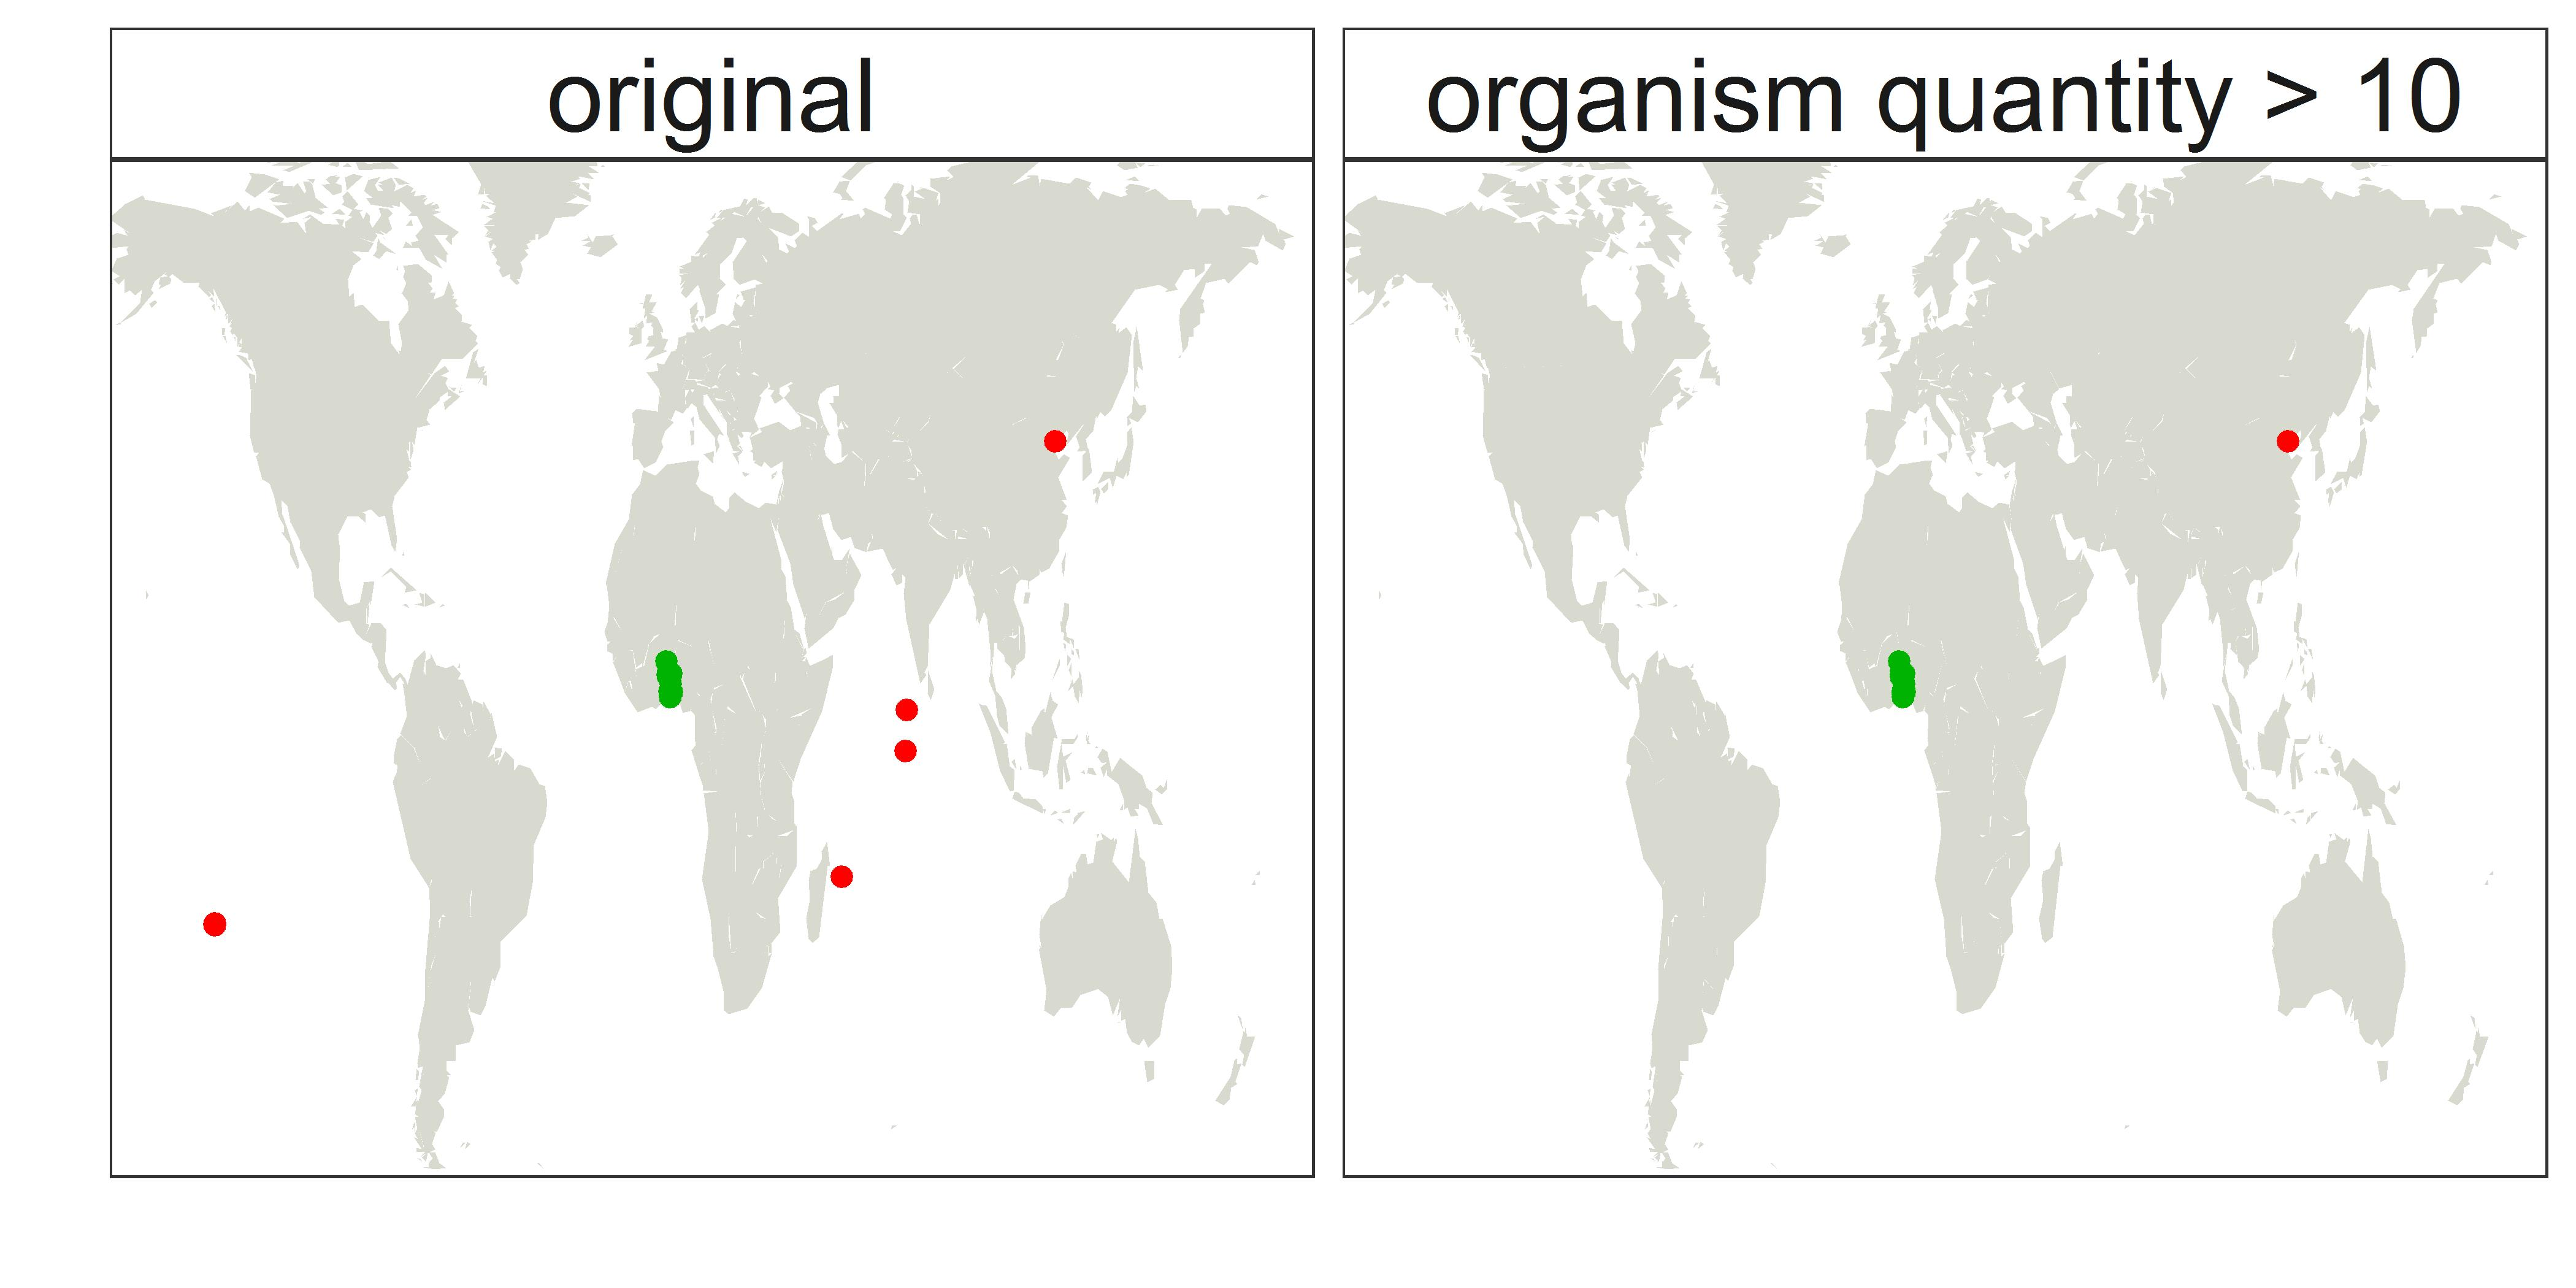
\includegraphics{/post/2020-01-08-metagenomics-occurrences-on-gbif_files/comparison_plot_1420595.jpg}

\hypertarget{moth}{%
\subsubsection{Moth}\label{moth}}

\begin{itemize}
\tightlist
\item
  link to
  \href{https://www.gbif.org/occurrence/map?taxon_key=1787267}{gbif map}
\item
  One {metagenomic point} might be legitimate point.
\end{itemize}

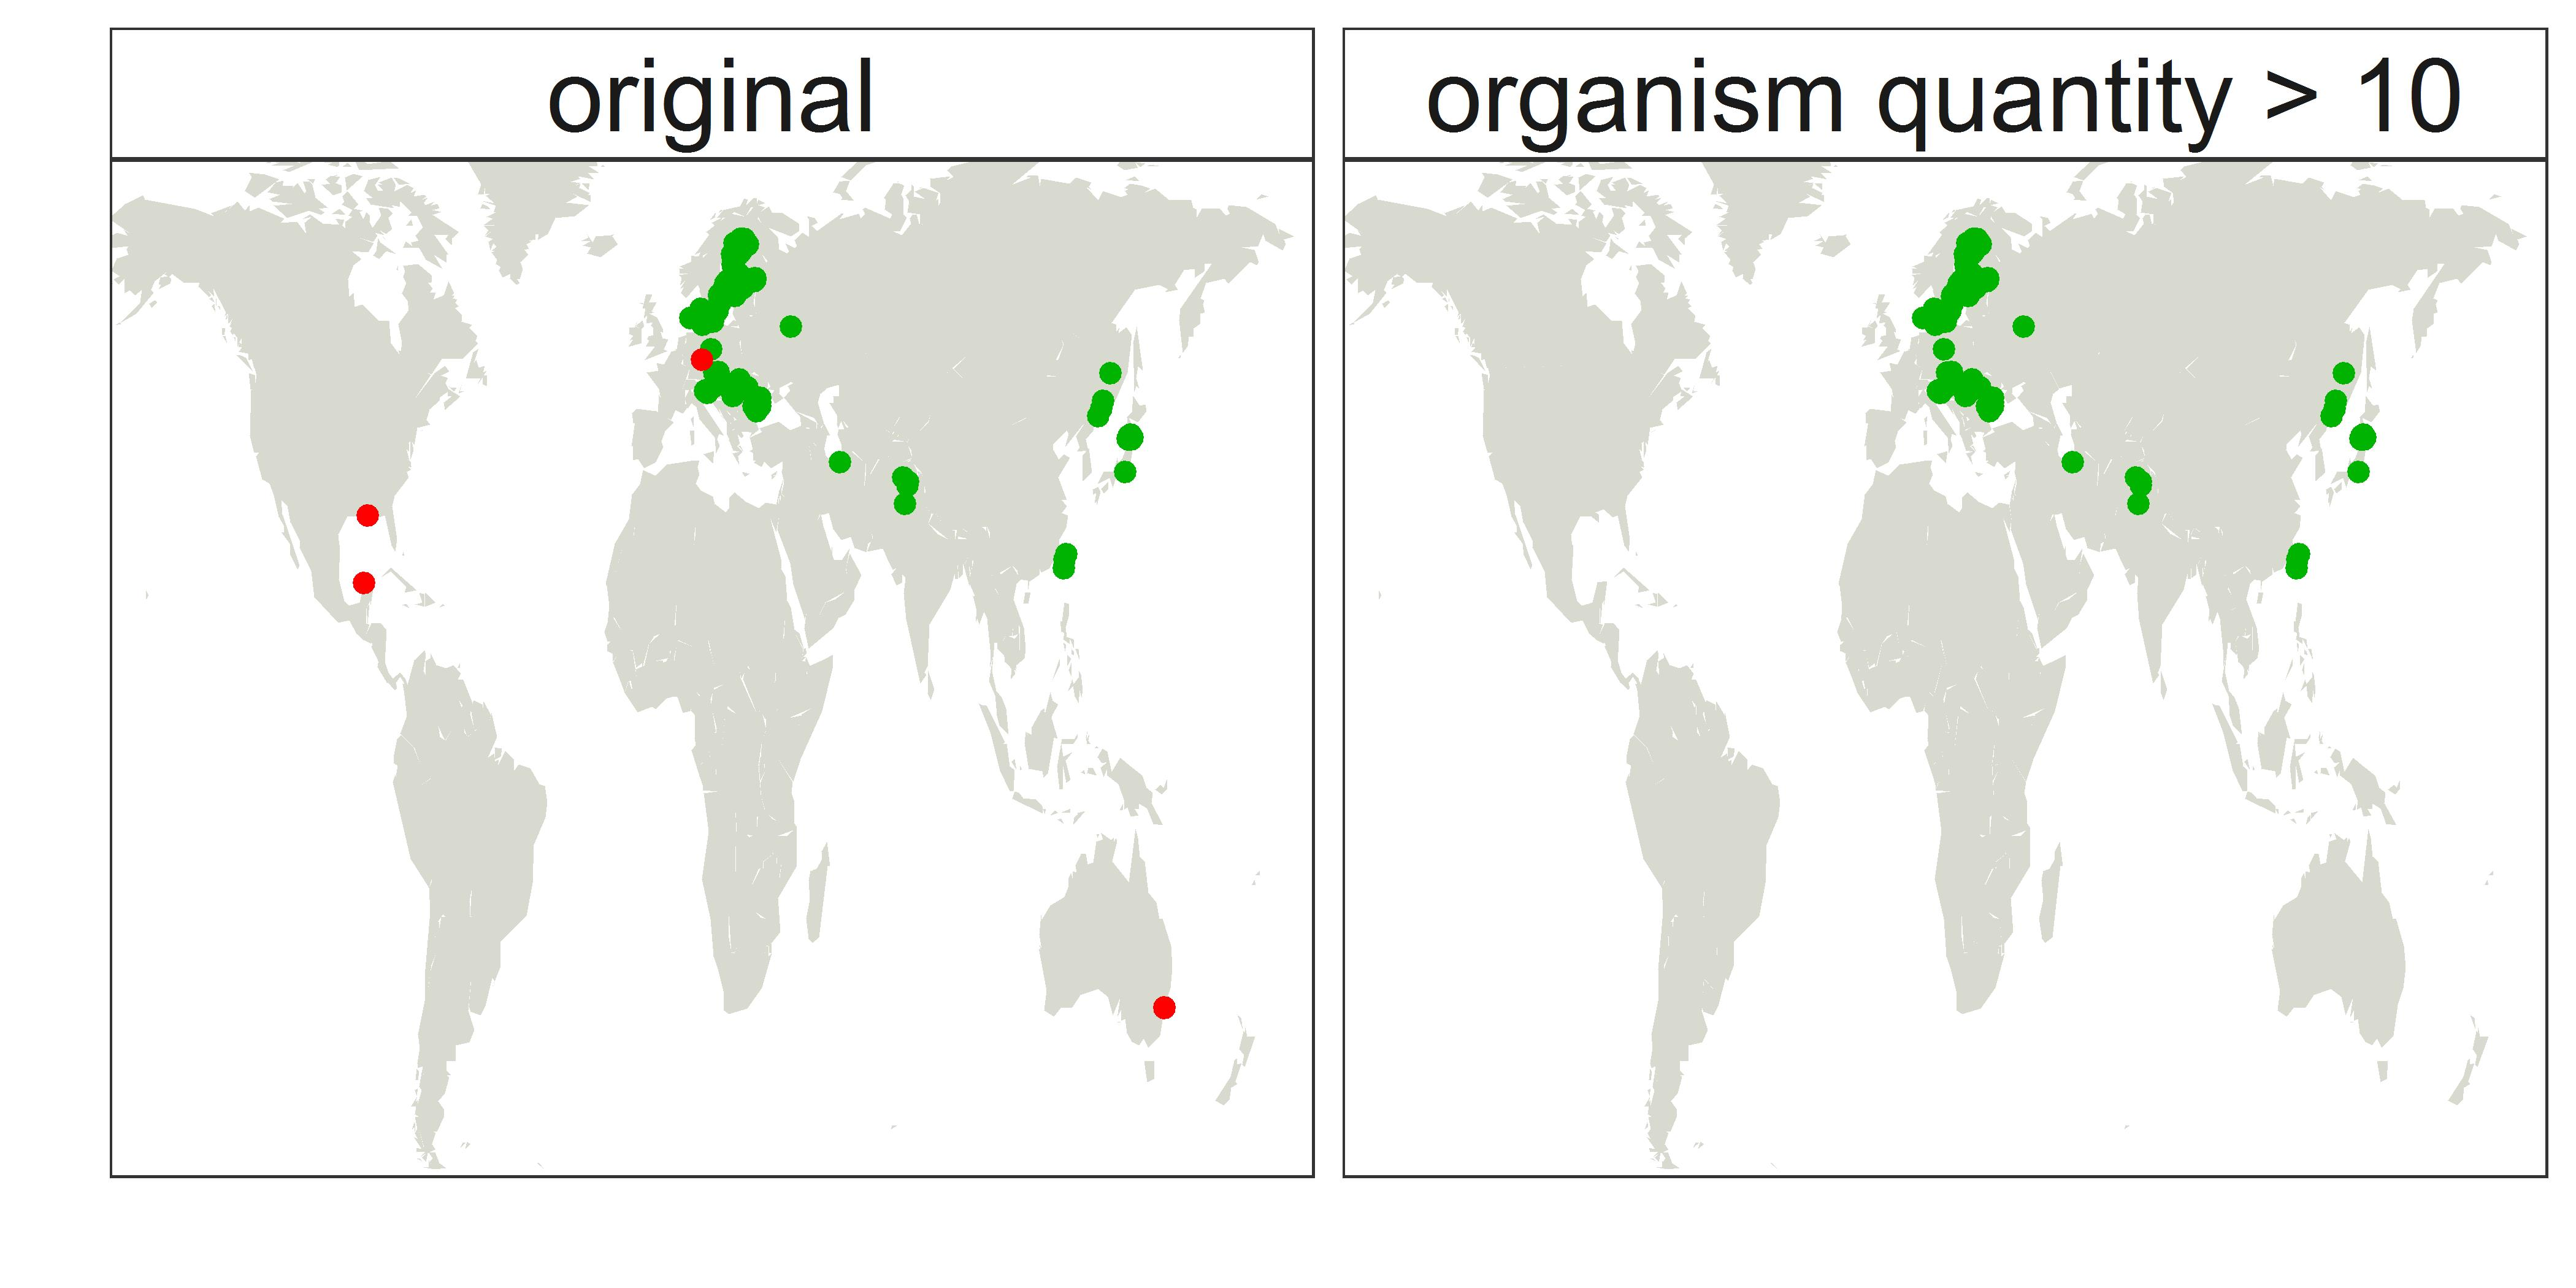
\includegraphics{/post/2020-01-08-metagenomics-occurrences-on-gbif_files/comparison_plot_1787267.jpg}

\hypertarget{house-pseudoscorpion}{%
\subsubsection{House pseudoscorpion}\label{house-pseudoscorpion}}

\begin{itemize}
\tightlist
\item
  link to
  \href{https://www.gbif.org/occurrence/map?taxon_key=5167813}{gbif map}
\item
  Hard to tell if {metagenomics points} points are outliers
\end{itemize}

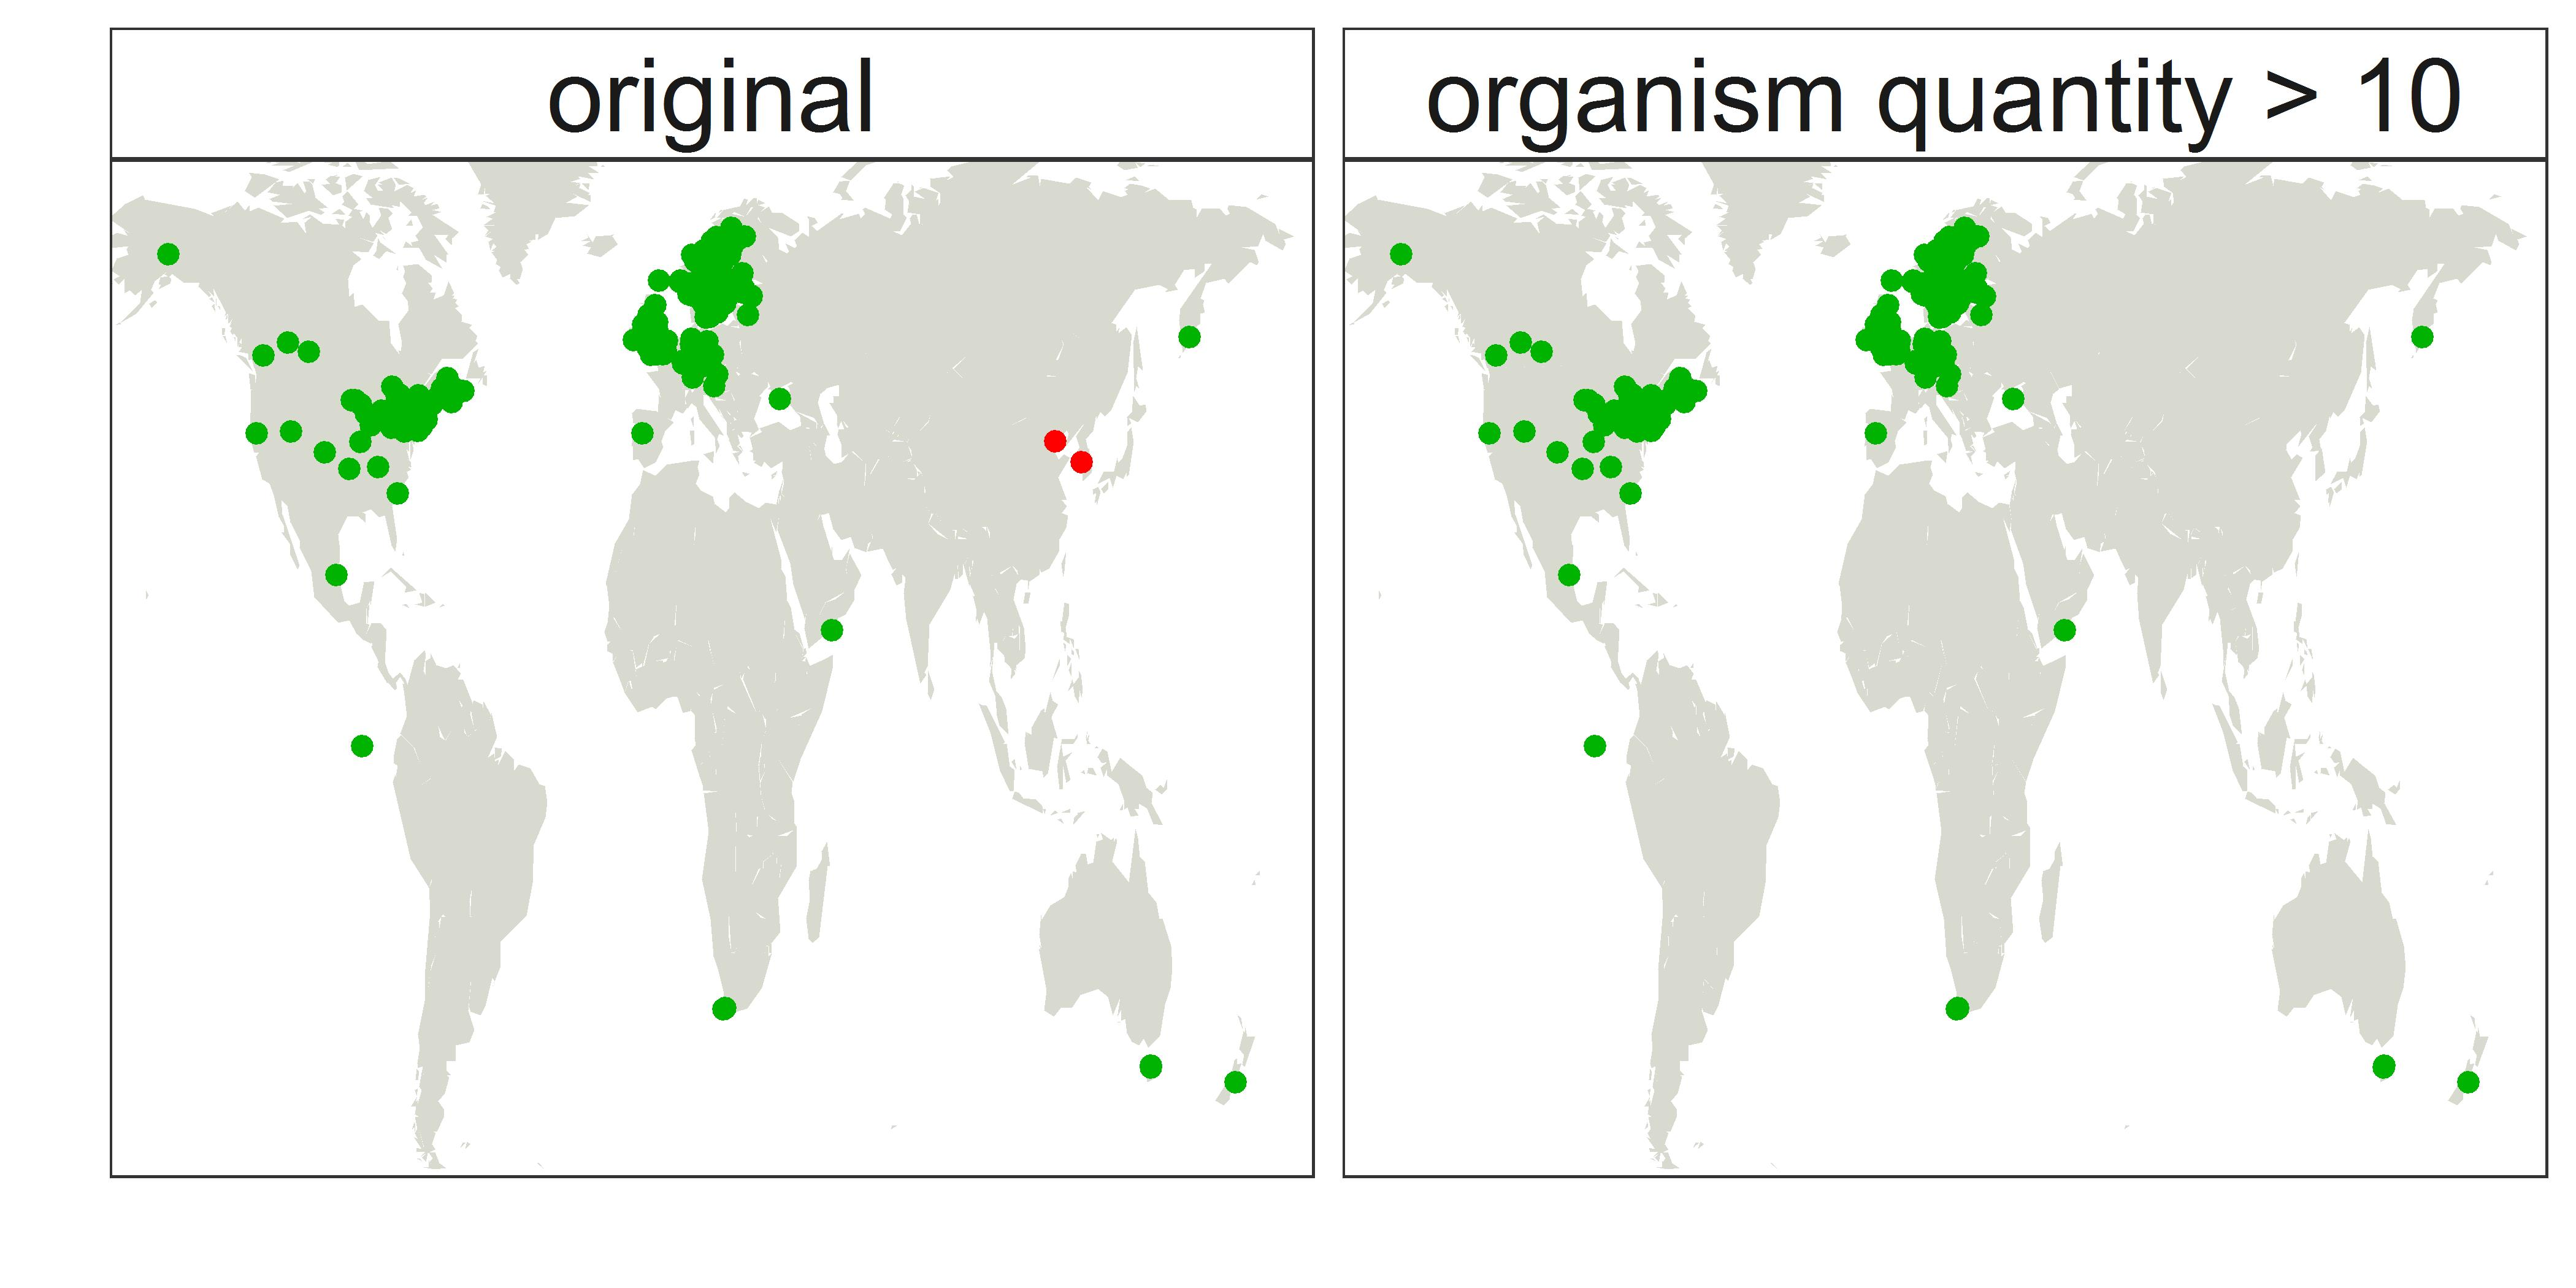
\includegraphics{/post/2020-01-08-metagenomics-occurrences-on-gbif_files/comparison_plot_5167813.jpg}

\hypertarget{there-are-less-than-10-birds-mammals-reptiles-amphibian-species-in-mgnify}{%
\section{There are less than 10 Birds, Mammals, Reptiles, Amphibian
species in
MGnify}\label{there-are-less-than-10-birds-mammals-reptiles-amphibian-species-in-mgnify}}

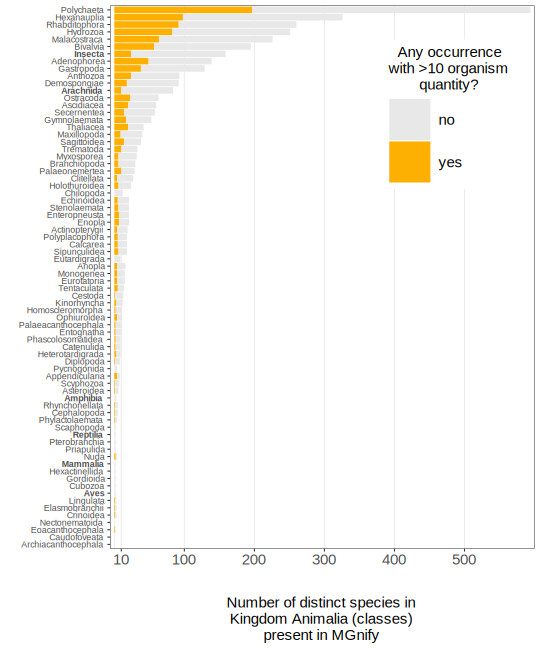
\includegraphics{/post/2020-01-08-metagenomics-occurrences-on-gbif_files/species_counts_barplot_with_filter.svg}

Since not many occurrences in MGnify are at rank species, there are not
many familiar animals in MGnify.

\hypertarget{species-counts-by-insect-order}{%
\section{Species counts by Insect
order}\label{species-counts-by-insect-order}}

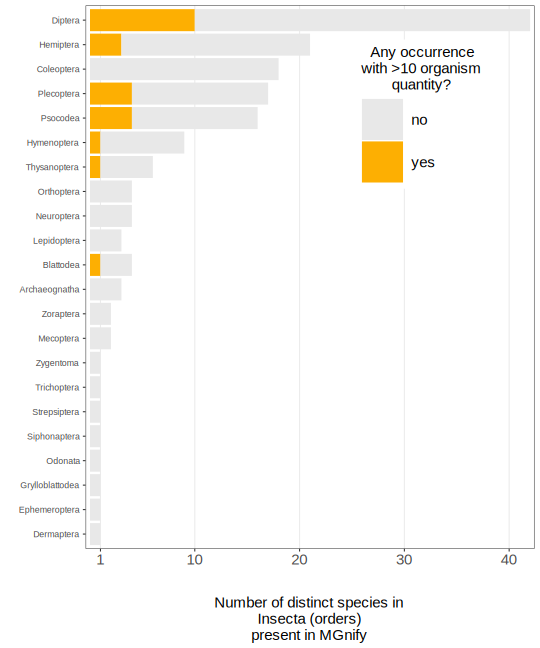
\includegraphics{/post/2020-01-08-metagenomics-occurrences-on-gbif_files/species_counts_barplot_with_filter_insects.svg}

\hypertarget{species-counts-by-plant-class}{%
\section{Species counts by Plant
class}\label{species-counts-by-plant-class}}

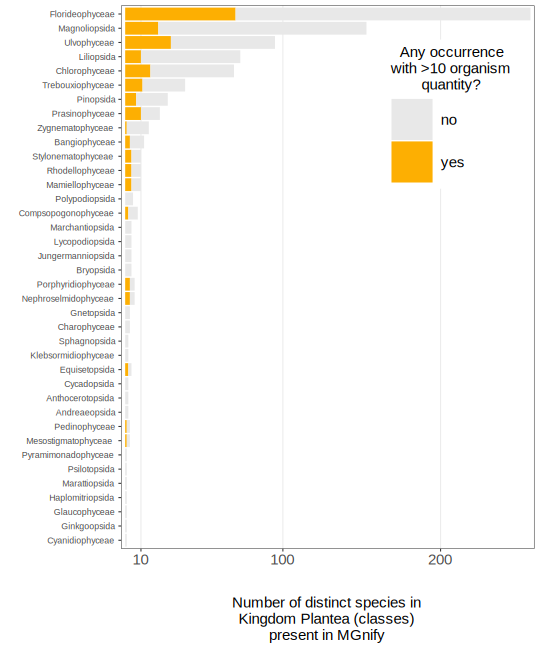
\includegraphics{/post/2020-01-08-metagenomics-occurrences-on-gbif_files/species_counts_barplot_with_filter_plants.svg}

Florideophyceae (the class with red algea) is the class with the most
species in MGnify

\hypertarget{plant-outlier-examples}{%
\section{Plant Outlier Examples:}\label{plant-outlier-examples}}

Other {GBIF datasets} in green and {Metagenomics datasets} plotted in
red.

\hypertarget{eastern-red-cedar}{%
\subsubsection{Eastern red cedar}\label{eastern-red-cedar}}

\begin{itemize}
\tightlist
\item
  link to
  \href{https://www.gbif.org/occurrence/map?taxon_key=2684391}{gbif map}
\item
  Hard to tell if {metagenomics points} are legitimate.
\item
  Most points have very little organism quantity backing them up.
\item
  Would be hard for naive user to know how to interpret this.
\end{itemize}

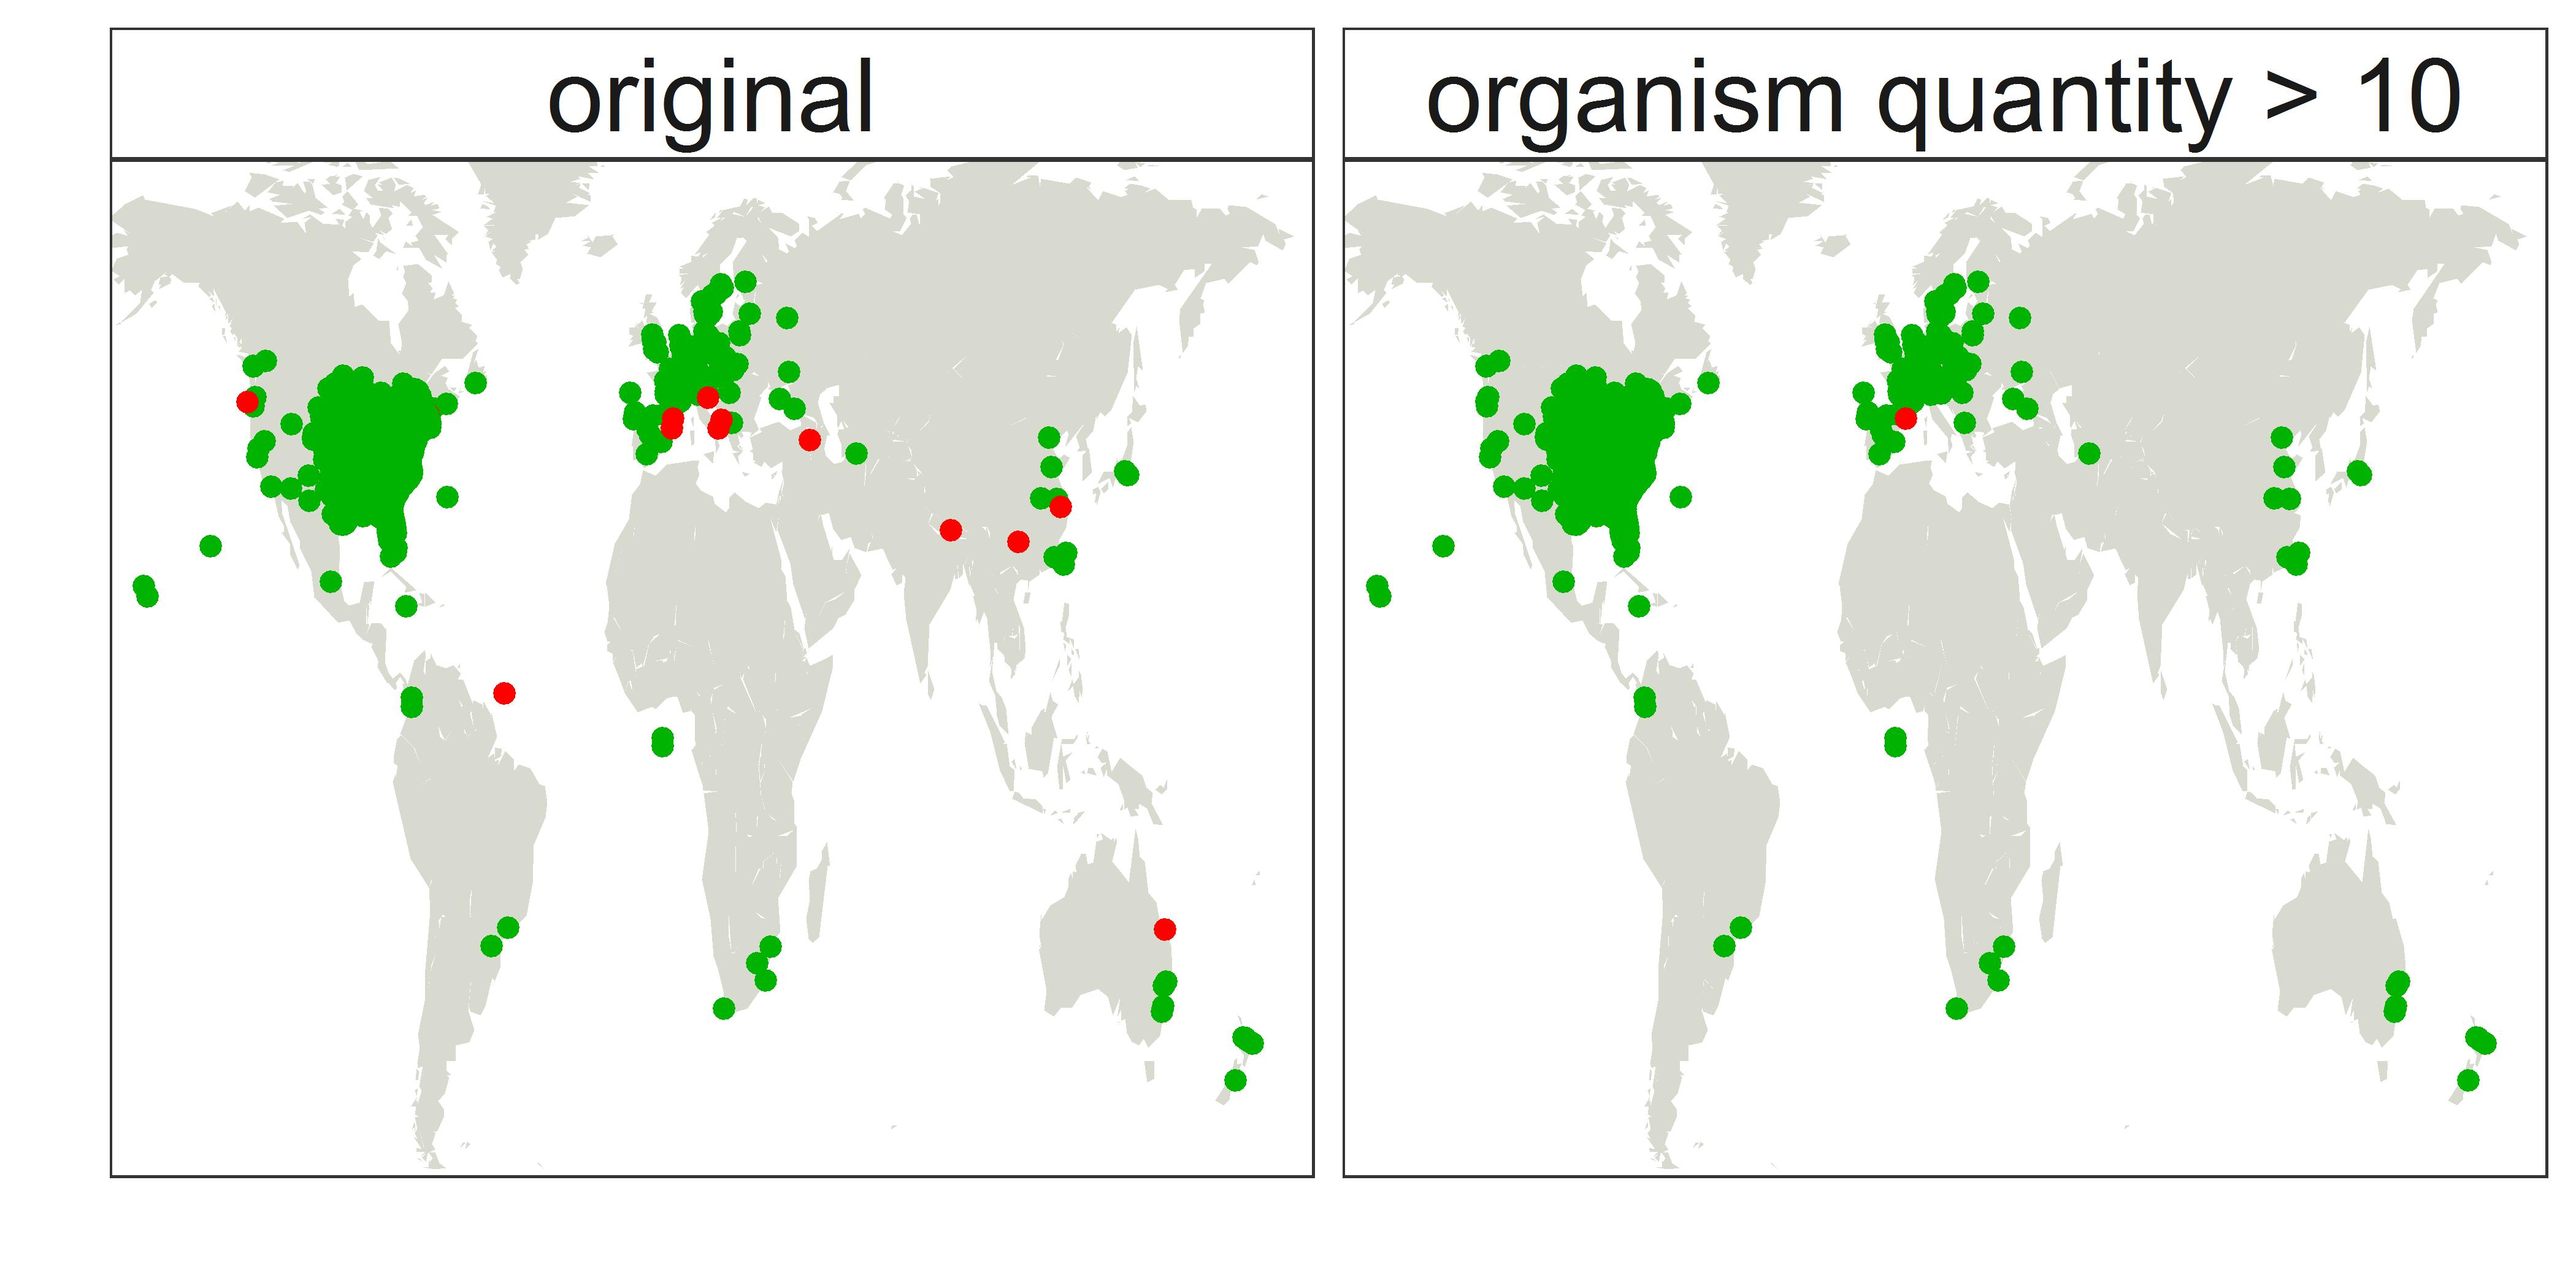
\includegraphics{/post/2020-01-08-metagenomics-occurrences-on-gbif_files/comparison_plot_2684391.jpg}

\hypertarget{campynemanthe-viridiflora}{%
\subsubsection{Campynemanthe
viridiflora}\label{campynemanthe-viridiflora}}

\begin{itemize}
\tightlist
\item
  link to
  \href{https://www.gbif.org/occurrence/map?taxon_key=2750616}{gbif map}
\item
  Endemic herb of New Caledonia (where all the green points are located)
\item
  All {metagenomics points} are very suspect.
\end{itemize}

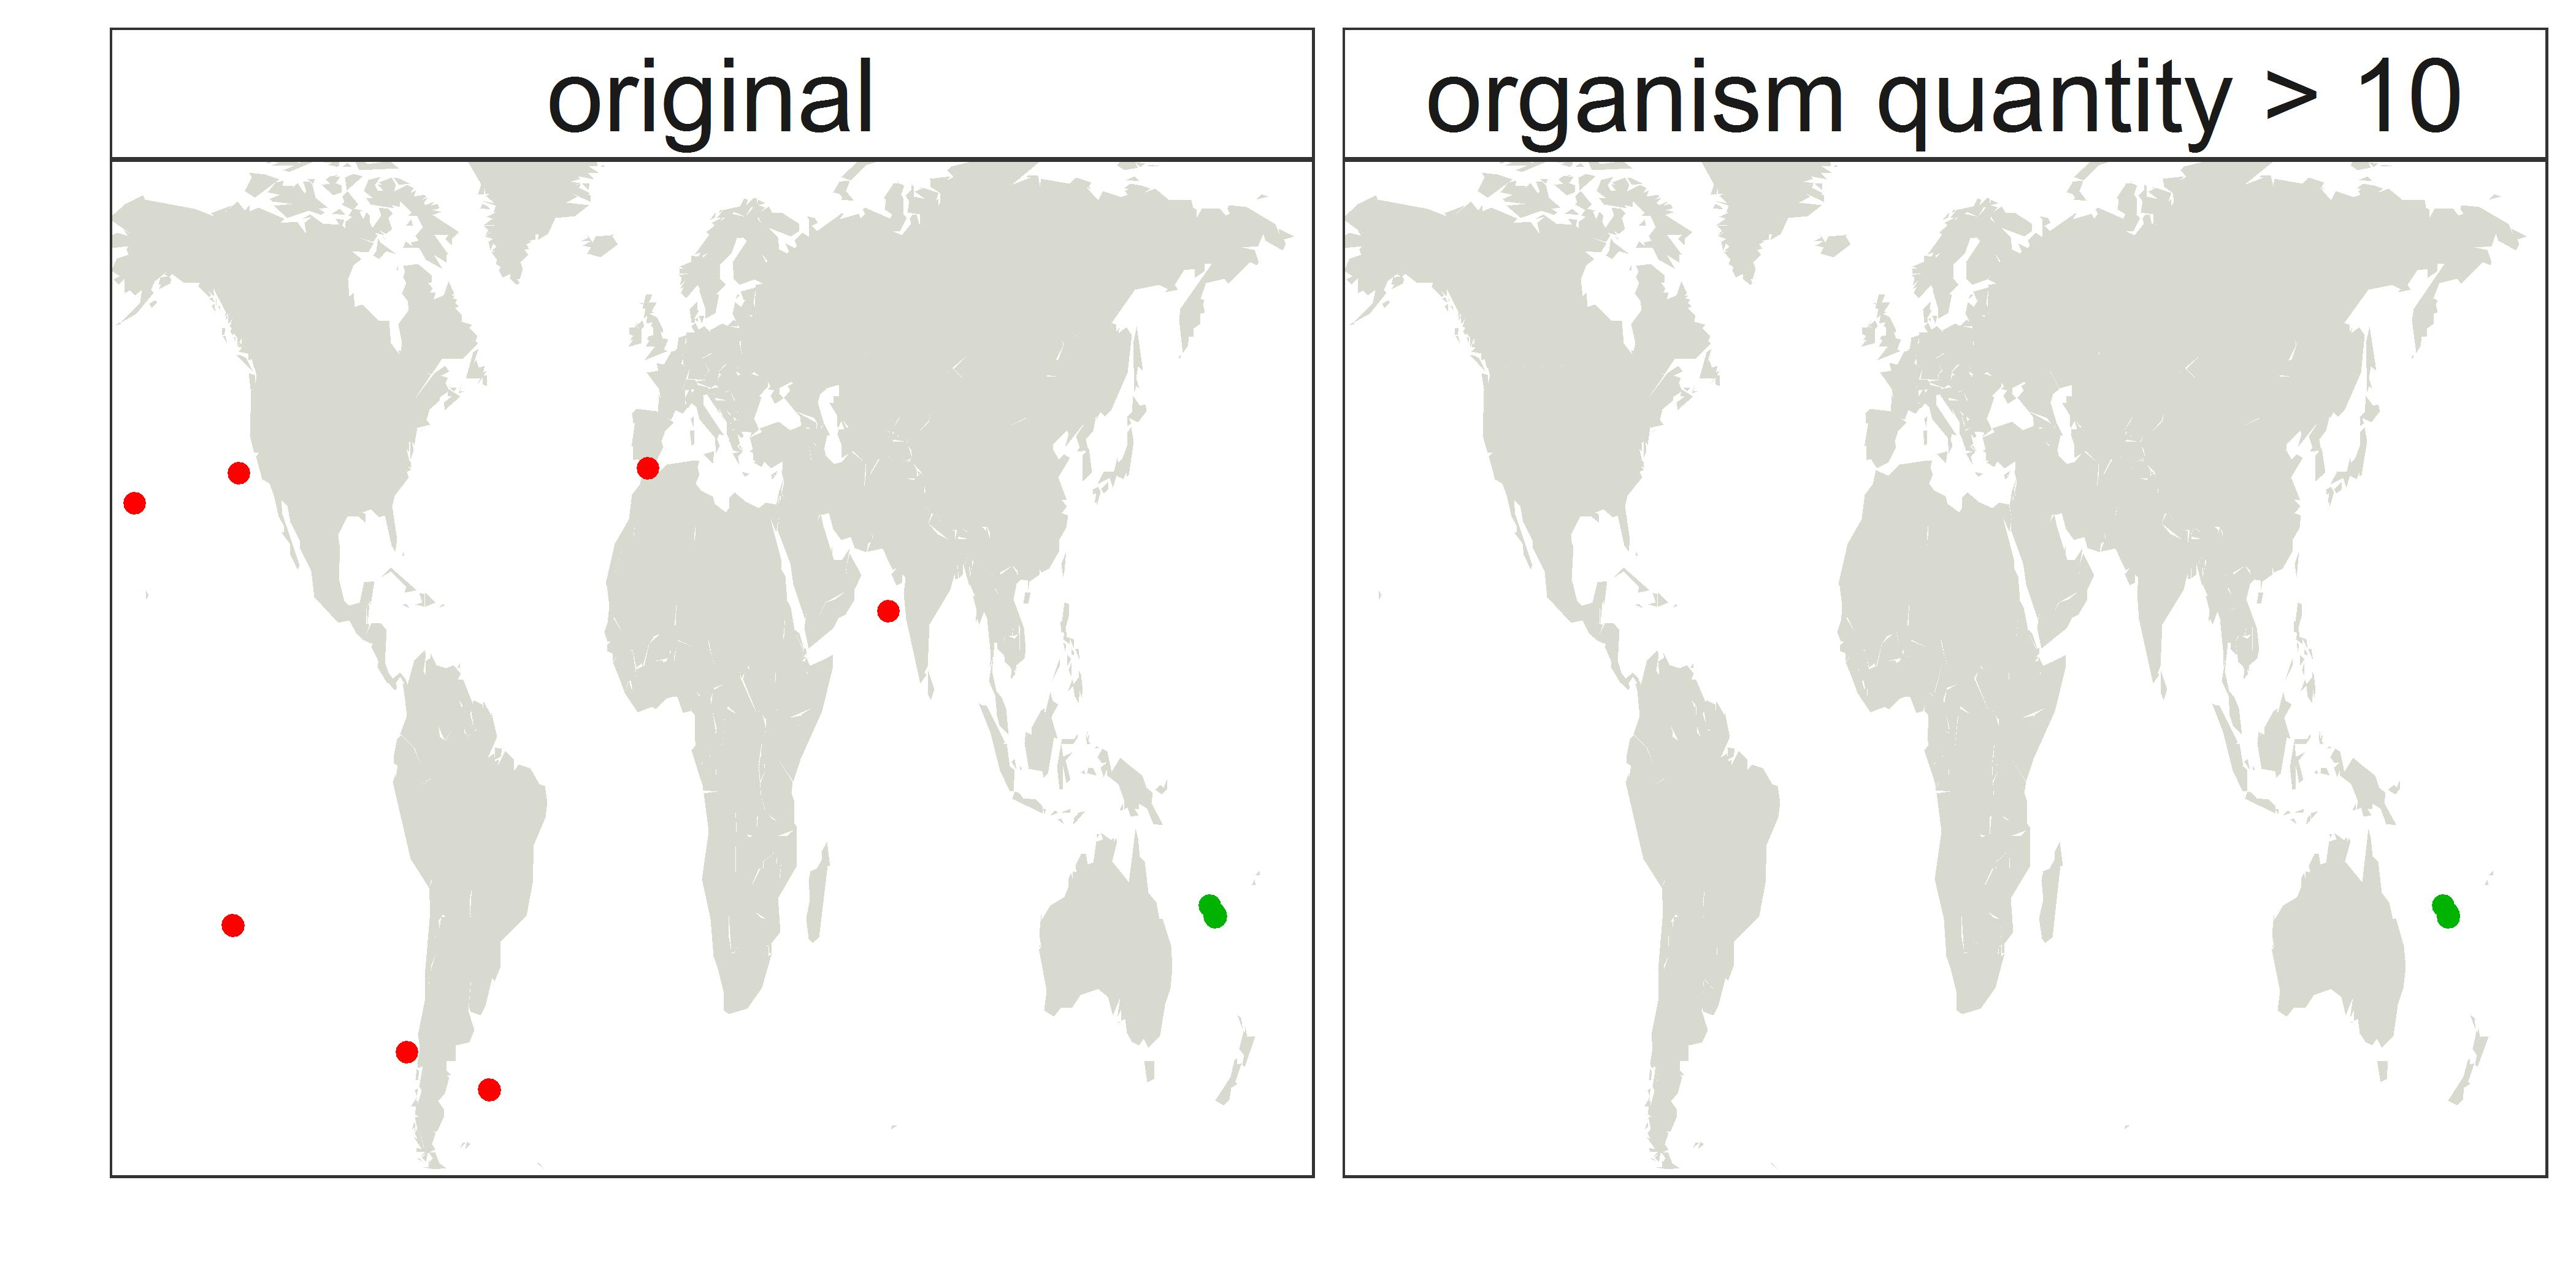
\includegraphics{/post/2020-01-08-metagenomics-occurrences-on-gbif_files/comparison_plot_2750616.jpg}

\hypertarget{quercus-lobata-valley-oak}{%
\subsubsection{Quercus lobata (Valley
oak)}\label{quercus-lobata-valley-oak}}

\begin{itemize}
\tightlist
\item
  link to
  \href{https://www.gbif.org/occurrence/map?taxon_key=2878373}{gbif map}
\item
  Many suspect {metagenomics points}!!
\item
  Other points also seem outside the natural range.
\item
  \href{https://www.gbif.org/occurrence/1091137039}{Point in New
  Zealand} from museum.\\
\item
  \href{https://www.gbif.org/occurrence/1846534143}{Point in Isreal}
  might be error.
\item
  \href{https://www.gbif.org/occurrence/2460559098}{Point in Spain}
  citizen science.
\item
  \href{https://www.gbif.org/occurrence/616369043}{Point in Germany} is
  a specimen from collection in Nuth. Probably not naturally occurring.
\item
  \href{https://www.gbif.org/occurrence/2014001054}{Point in Louisiana}
  has relatively high organism quantity at 0.0025.
\end{itemize}

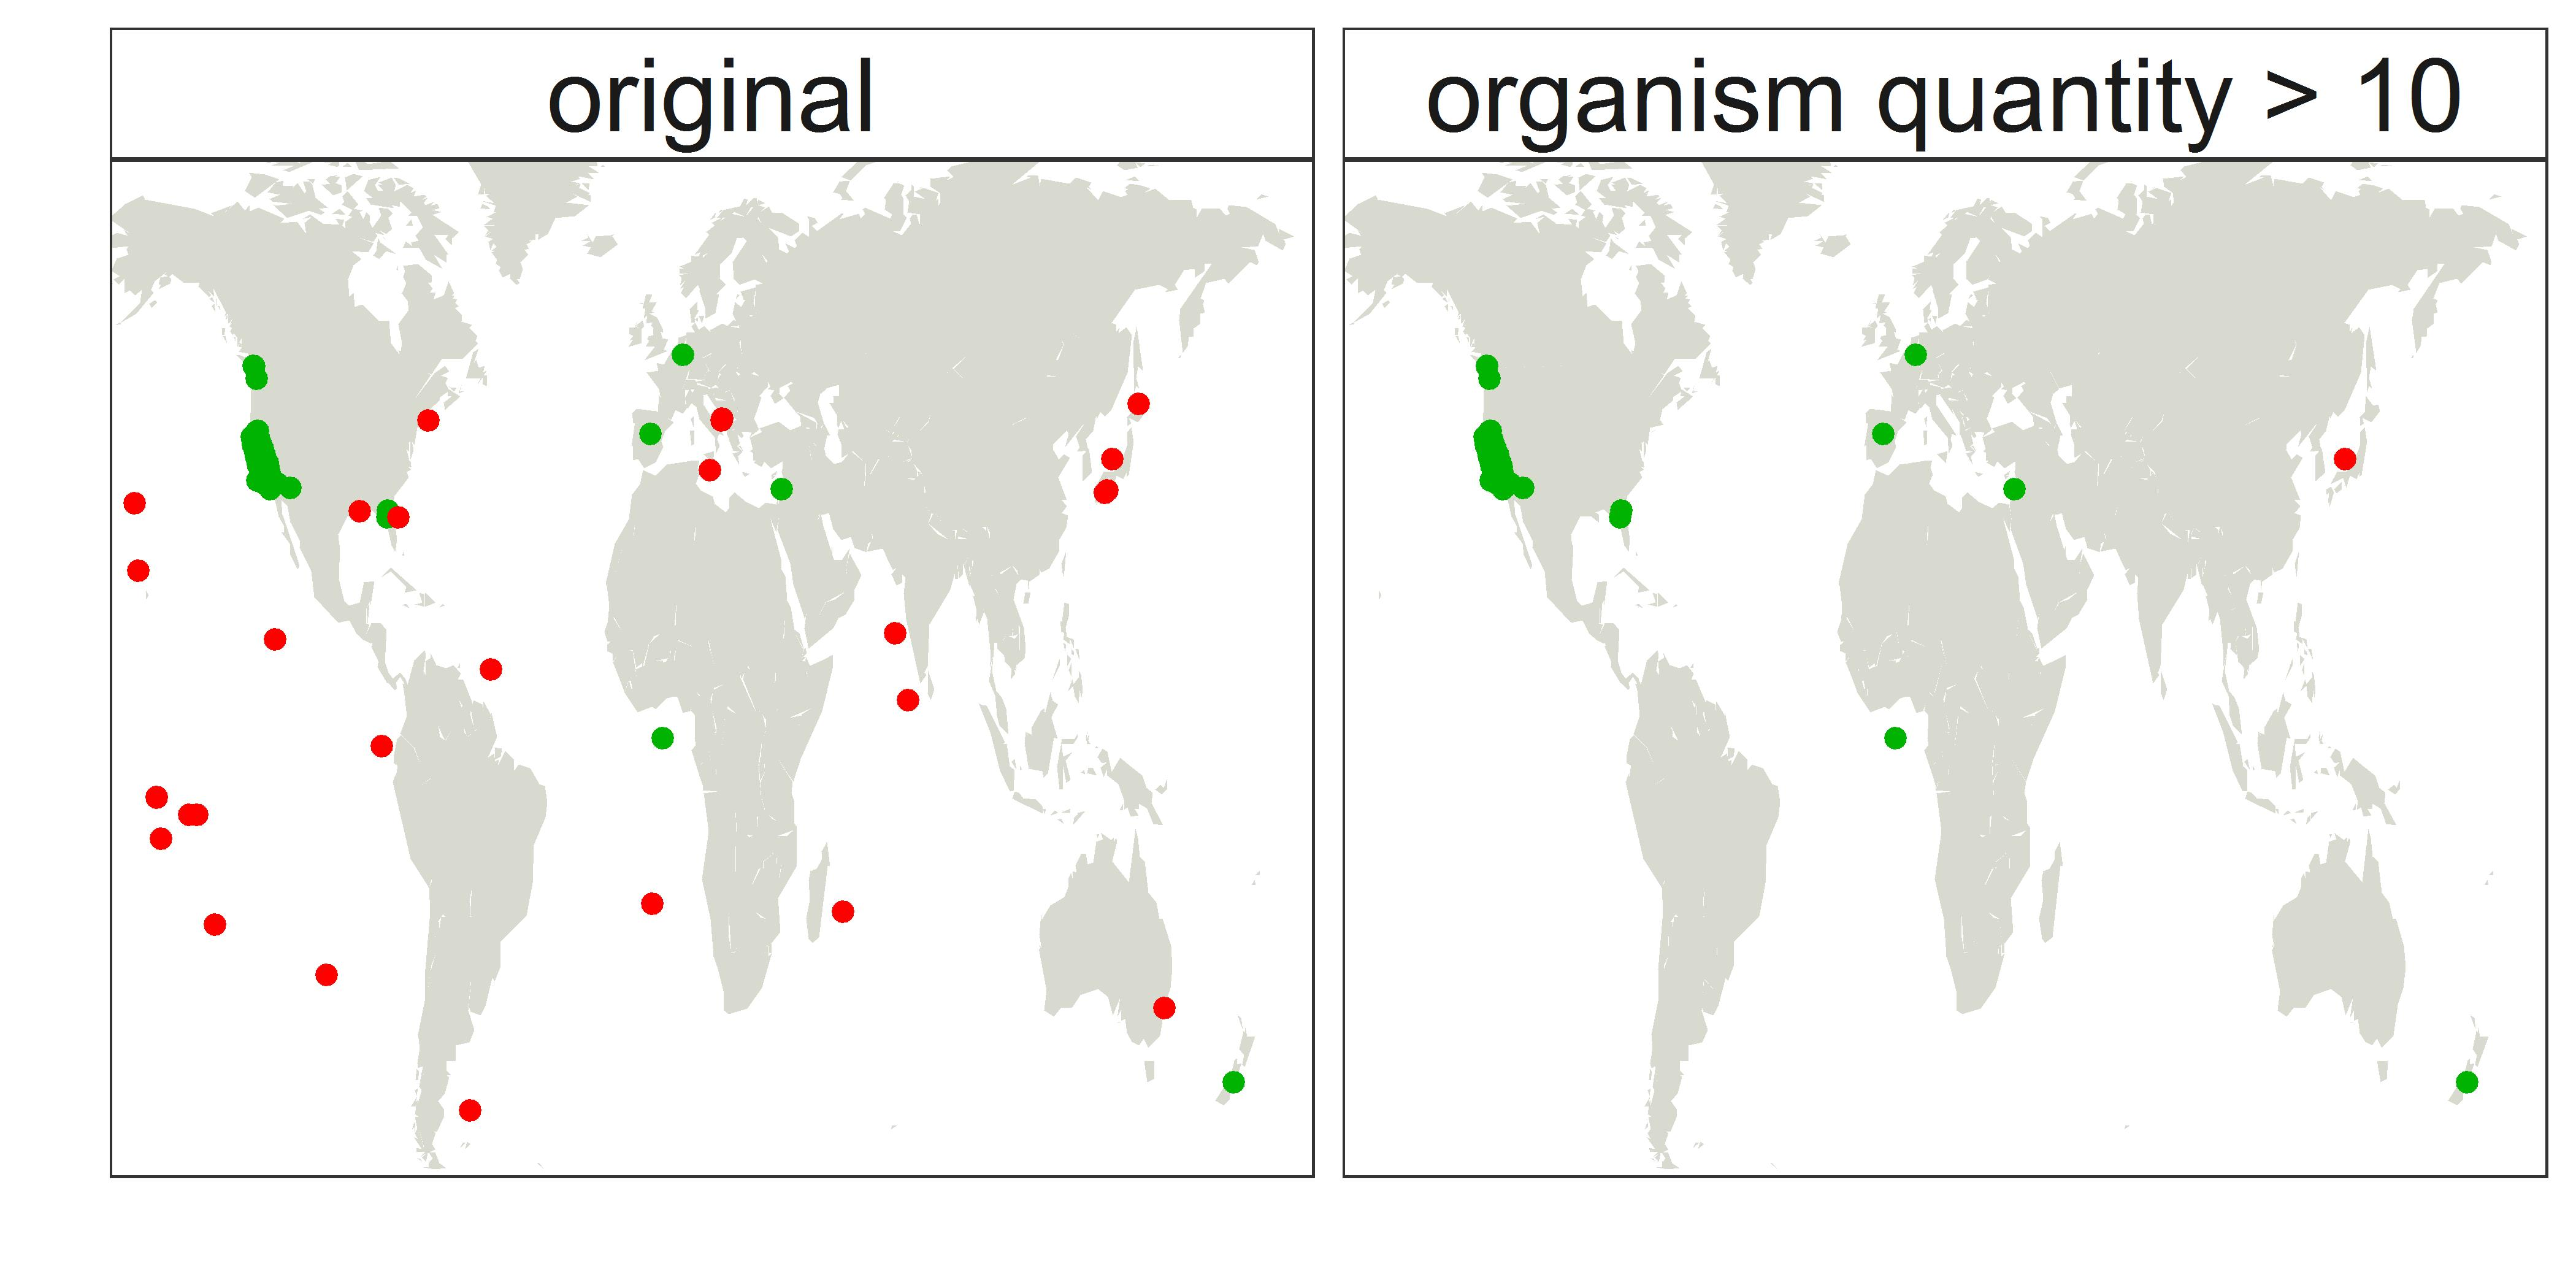
\includegraphics{/post/2020-01-08-metagenomics-occurrences-on-gbif_files/comparison_plot_2878373.jpg}

\hypertarget{adiantum-pedatum-northern-maidenhair-fern}{%
\subsubsection{Adiantum pedatum (Northern maidenhair
fern)}\label{adiantum-pedatum-northern-maidenhair-fern}}

\begin{itemize}
\tightlist
\item
  link to
  \href{https://www.gbif.org/occurrence/map?taxon_key=2651832}{gbif map}
\item
  {metagenomics points} seem plausible, but none pass a very
  conservative filter of \textgreater{}10 organsism quanity.
\item
  \href{https://www.gbif.org/occurrence/2273846947}{point in South
  America} might be specimen in museum.
\end{itemize}

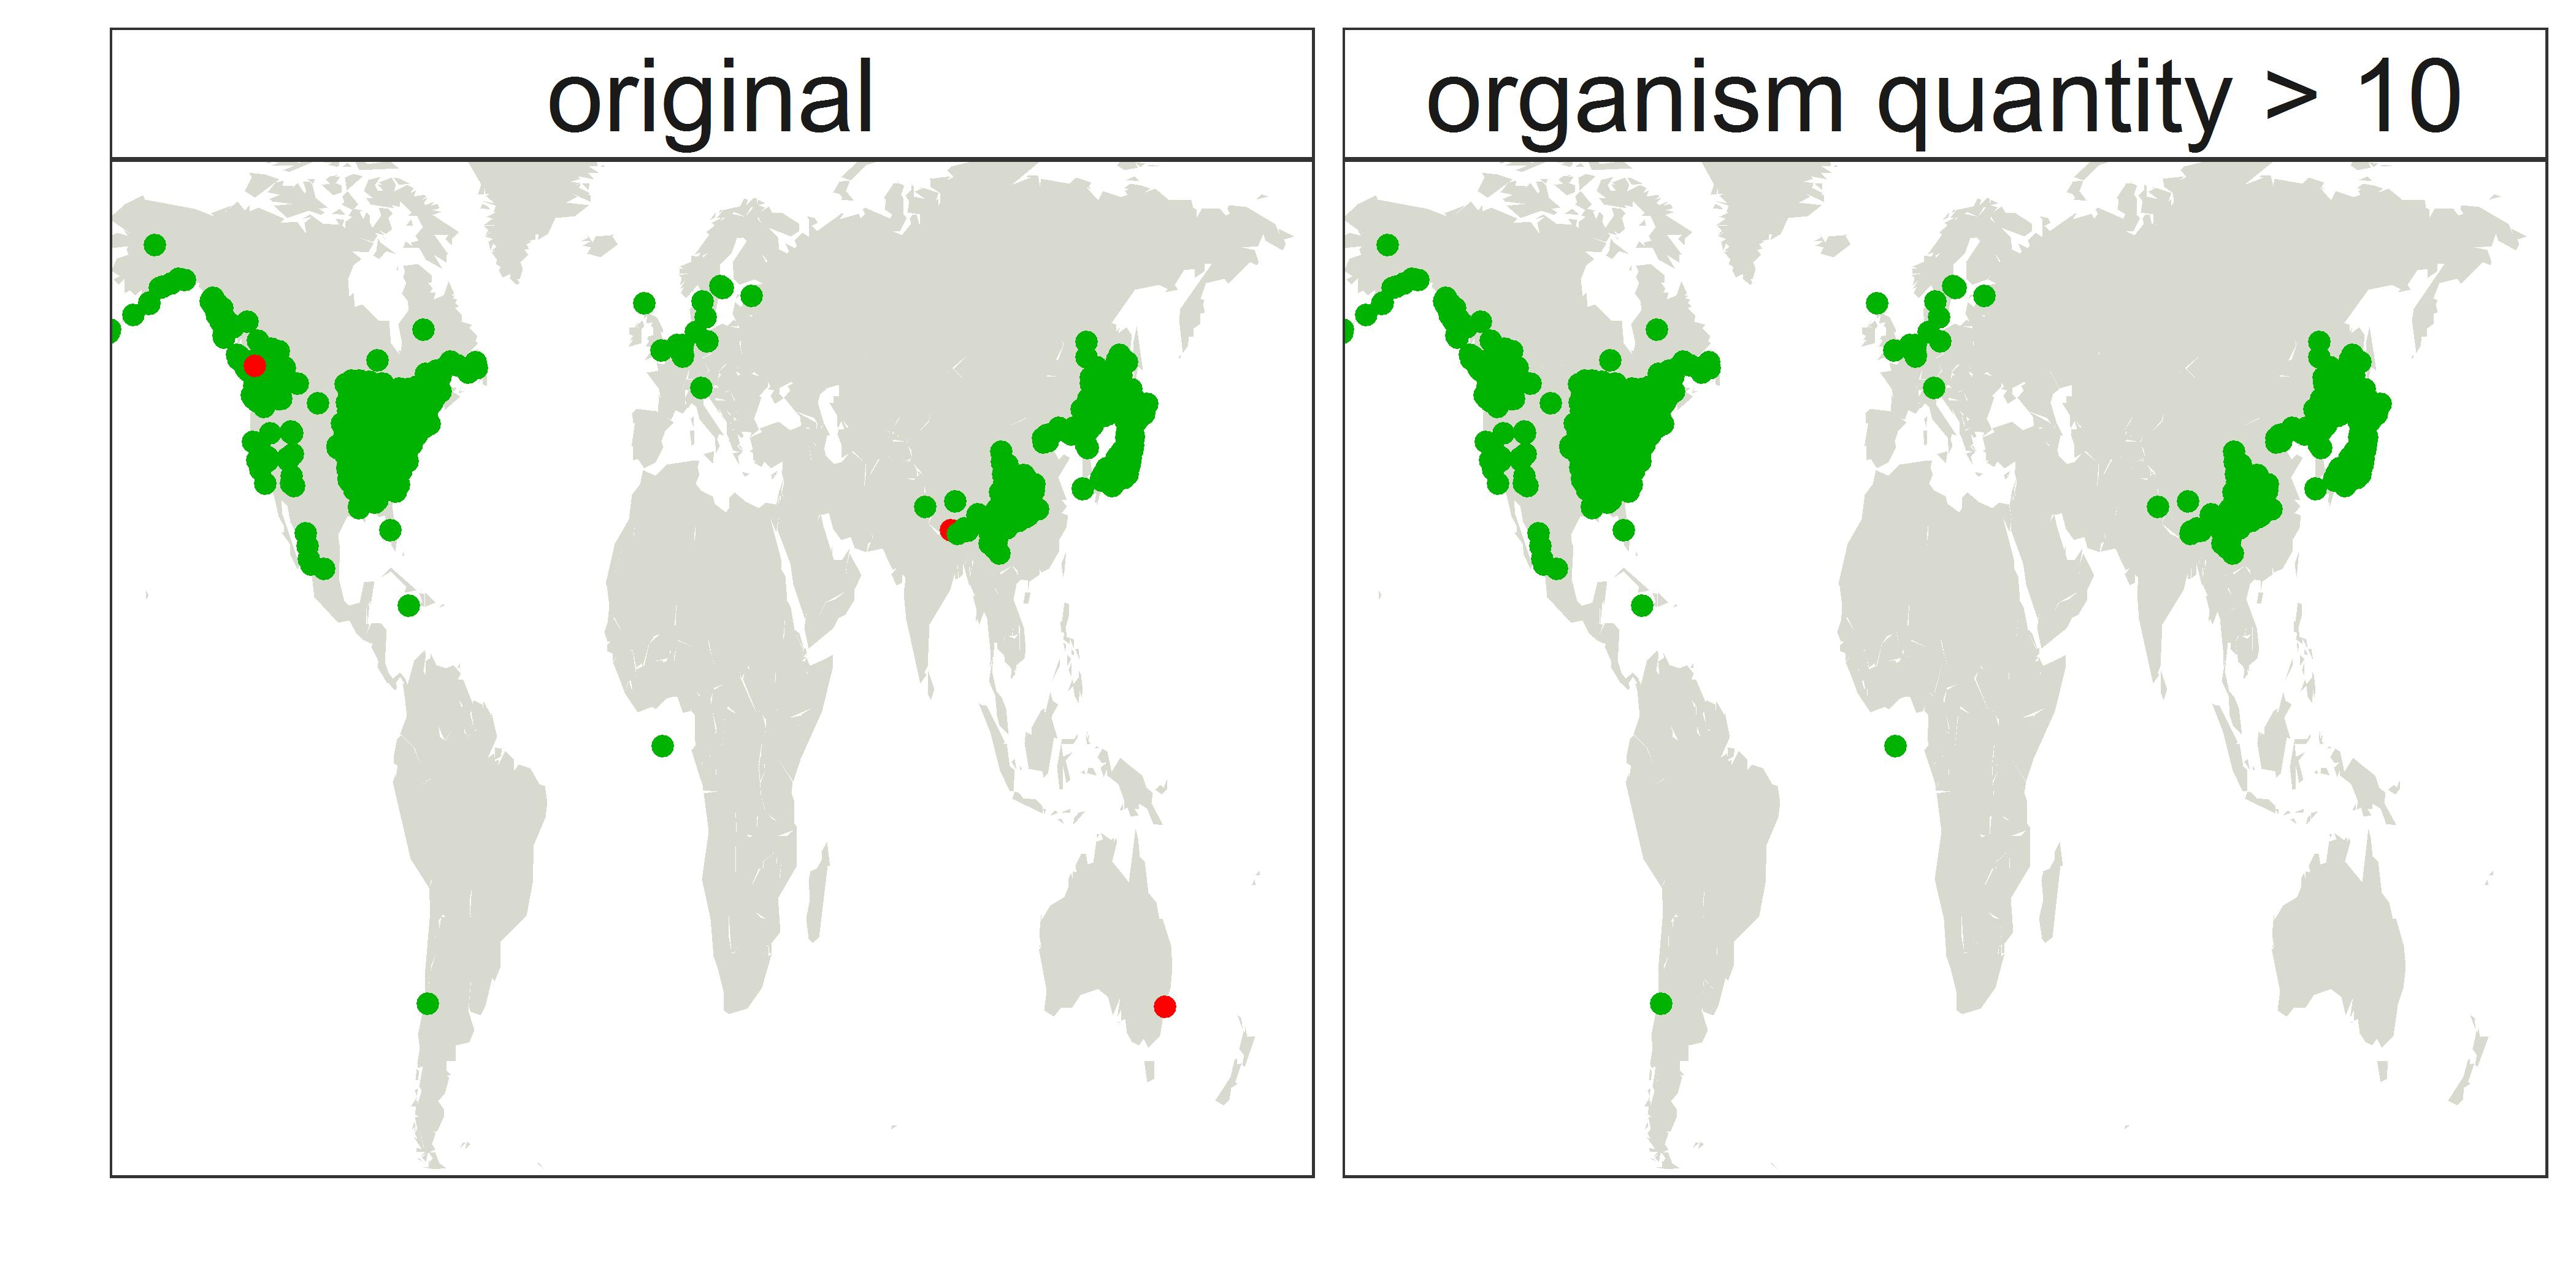
\includegraphics{/post/2020-01-08-metagenomics-occurrences-on-gbif_files/comparison_plot_2651832.jpg}

\hypertarget{what-is-the-right-cut-off}{%
\section{What is the right cut off?}\label{what-is-the-right-cut-off}}

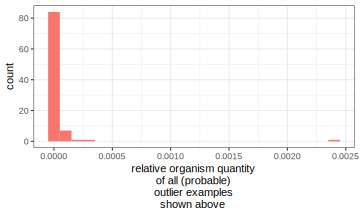
\includegraphics{/post/2020-01-08-metagenomics-occurrences-on-gbif_files/probable_outlier_examples.svg}

Here we see that a educated guess for the ``right cut off'' for relative
organism quantity is something around \textbf{\textgreater{}0.0005 or
\textgreater{}0.0025.} \textbf{I excluded Eastern Red Cedar} from this
plot, since it was the example with the most plausible points (although
none its points had a relative organism quanity \textgreater{}0.0025).

\begin{itemize}
\tightlist
\item
  \href{https://www.gbif.org/occurrence/2014001054}{Point in Louisiana}
  has relatively high organism quantity at 0.0025.
\end{itemize}

\hypertarget{what-happens-when-we-use-a-cutoff-of-0.0025}{%
\section{What happens when we use a cutoff of
0.0025?}\label{what-happens-when-we-use-a-cutoff-of-0.0025}}

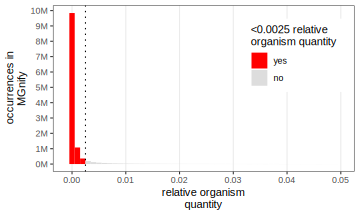
\includegraphics{/post/2020-01-08-metagenomics-occurrences-on-gbif_files/relative_organism_quantity.svg}

\begin{itemize}
\tightlist
\item
  This \textbf{filter excludes 90\% of MGnify occurrences}.
\end{itemize}

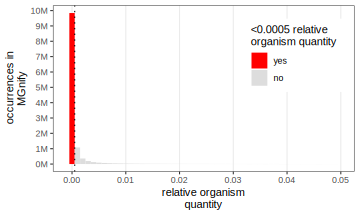
\includegraphics{/post/2020-01-08-metagenomics-occurrences-on-gbif_files/relative_organism_quantity_0.0005.svg}

\begin{itemize}
\tightlist
\item
  This \textbf{filter excludes 80\% of MGnify occurrences}.
\end{itemize}

Experimental filter implemented at:

\url{https://www.gbif-dev.org/}

\hypertarget{rod-page-example-cricket-at-rank-genus}{%
\section{Rod Page Example Cricket at rank
Genus}\label{rod-page-example-cricket-at-rank-genus}}

Paroecanthus Saussure, 1859

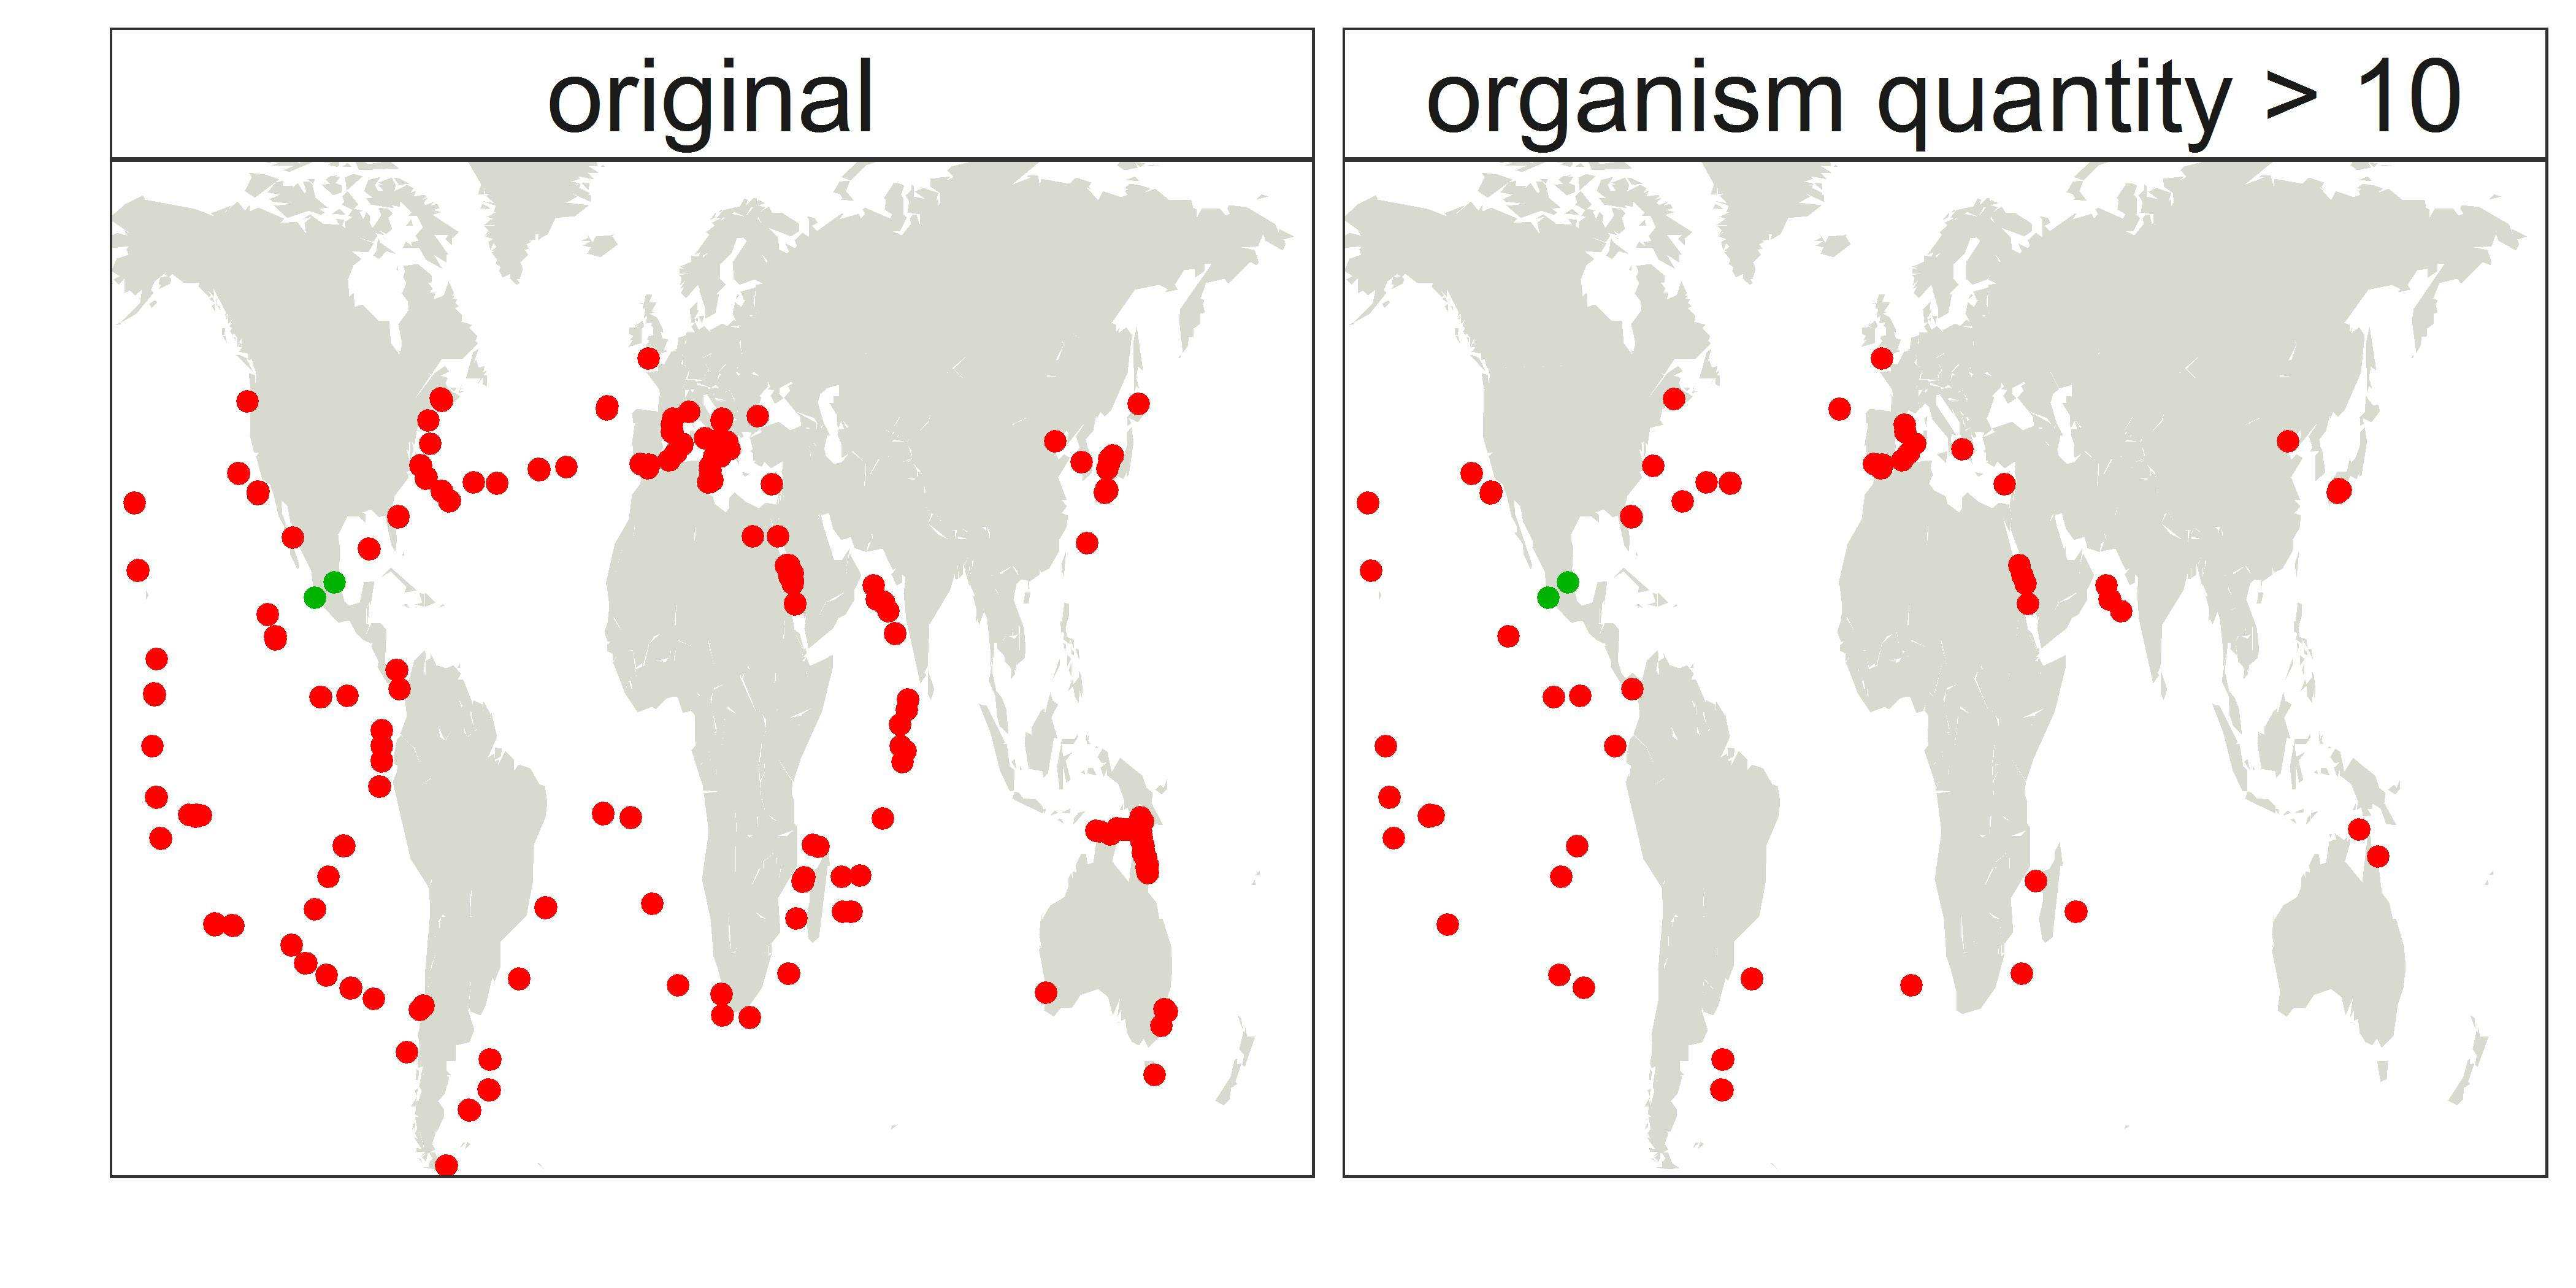
\includegraphics{/post/2020-01-08-metagenomics-occurrences-on-gbif_files/comparison_plot_6758530.jpg}

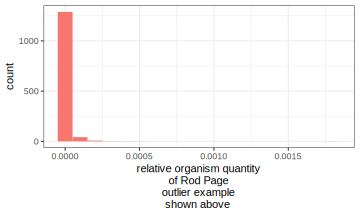
\includegraphics{/post/2020-01-08-metagenomics-occurrences-on-gbif_files/rod_page_example.svg}

\end{document}
